Linguistic rules capture two types of generalizations: \textbf{well-formedness conditions}, i.e.\ the requirements for a word to be well-formed, and \textbf{transformations}, i.e.\ the rules of re-computing the given underlying representation into the corresponding surface form.
The former restrict the word's form itself, such as ``two vowels should never be adjacent to each other'', while the latter describe the change, such as ``insert {[}j{]} in-between two adjacent vowels''.
For example, transformations map the Russian word that is orthographically represented as \emph{dlinnosheee} `long-necked' into its pronunciation \emph{dlinnosh[ejeje]}, and the well-formedness conditions ensure that the pronunciation \emph{dlinnosh[eee]} is not allowed since it contains two vowels adjacent to each other.


\textbf{Grammars} describe how to build well-formed words from the elements of the \textbf{alphabet}.
A \textbf{language} of the grammar is a potentially infinite collection of all well-formed strings of that grammar.
Thus in a formal sense, it simply refers to a collection of words, or \textbf{strings}.
\textbf{Transformations} are functions from the input language, i.e.\ a collection of ``underlying representations'', onto the output language, or a collection of ``surface forms''.


In this chapter, I discuss \emph{subregular grammars} (Section~\ref{wellformednesssection}) and \emph{subsequential functions} (Section~\ref{modelingtransofrmationsection}) as they seem to be a good fit for natural language dependencies \citep[i.a.]{Heinz11part1,HeinzRawal11,GainorLai12,Heinz-Lai-2013-VHS,AksenovaEtAl16,Graf17CLSpres,ChandleeHeinz2018}.
In the two following chapters, I show the results of the \emph{automatic extraction} of subregular grammars and subsequential functions given the learning framework defined in Section \ref{learningframework}.


\section{Modeling well-formedness conditions}
\label{wellformednesssection}

To model well-formedness conditions means to find a way to discriminate between well-formed and ill-formed words of a language.
In other words, it implies finding a grammar that only builds well-formed strings, and that can recognize which strings are ill-formed.
For example, given the alphabet of vowels and consonants, a grammar can prohibit vowel hiatus by penalizing adjacent vowels.%
\footnote{Strictly speaking, grammars do not recognize if a string is well-formed, but rather provide a finite specification of the language.
Instead, a recognizer judges the well-formedness of strings.
However, for the sake of simplicity and conciseness, I do not separate these two notions in my dissertation.
}

Subregular grammars provide an interpretable and succinct way to encode such rules.
These grammars are very weak and restricted, however, they are sufficiently powerful for natural language.
Interestingly, the subregular nature of linguistic generalizations allows us to explain the absence of some theoretically possible yet typologically unattested patterns \citep{GainorLai12}; I come back to the issue of typology in Section~\ref{subgsgf}.
Also, this approach gives insights into human cognition since there is evidence that only some subregular language classes are learnable \citep{Lai15}.
As it follows from the name itself, subregular grammars are a subset of the regular ones, and therefore let us first establish the regular nature of natural language patterns.



\subsection{Regular nature of natural language patterns}
\label{regnatofnlpt}

Consider a pattern of Russian compounding, where a morpheme \emph{-o-}%
\footnote{This marker is also sometimes realized as \emph{-e-}.}
 is located in-between compounding stems.
For example, the stems \emph{vod(-a)}%
\footnote{\emph{-a} is a suffix marking nominative case, singular form for some nominal classes.}
 `water' and \emph{voz} `carrier' can be combined to obtain a complex word \emph{vod-o-voz} `water carrier'.
If the compound is composed of multiple stems, the marker is added in-between every one of them: \emph{vod-o-voz-o-voz} `carrier of water carriers'.

This pattern can be viewed as a language of well-formed sequences of stems and compounding affixes.
Strings such as \emph{stem}, \emph{stem-o-stem}, \emph{stem-o-stem-o-stem} belong to the target language, but \emph{stem-stem} and \emph{stem-o} do not.
This can be rephrased a rule ``a well-formed form cannot start or end with a compounding marker, and within a word, two markers or two stems should not be adjacent to each other''.
Generalizations like this can be conveniently expressed as finite state automata.

A \textbf{finite state automaton} (FSA) is a type of an abstract machine that is defined by a finite list of states and the transitions between those states \citep{Lawson2003}.
In the case of string-based automata, these transitions are annotated with characters.
An automaton reads a string of characters (the input string), and every new character changes the current state.
Some of the states are \textbf{initial}, meaning that the first character of the input string can be read from those states.
\textbf{Final}, or \emph{accepting} states are the ones that indicate that the string is accepted.
The input string is accepted by an automaton when the first character of that string can be read from the initial state, and this string is a path from the initial state to the final one.

Consider the automaton in Figure \ref{fig:ruscompounding}.
The numbered circles represent states, and the arrows are the transitions between those states.
States are usually referred to as $q$, therefore the states of that machine are $q_0$, $q_1$ and $q_2$. 
The initial state is represented with an incoming ``start'' arc.
The state $q_1$ is marked with a double circle, meaning that it is final.


\begin{figure}[h!]
\centering
\begin{tikzpicture}
    \node (0) [state, accepting] {$1$};
    \node (1) [state, right=of 0] {$2$};
    \node (2) [state, left=of 0, initial] {$0$};
    \path [-{Stealth[]}]
      (0) edge[bend left = 45] node [above] {-o-} (1)
      (1)  edge[bend left = 45] node [above] {stem} (0)
      (2) edge node [above] {stem} (0)
      ;
  \end{tikzpicture}
\caption{FSA for Russian compounding.}
\label{fig:ruscompounding}
\end{figure}


A language of an FSA is a potentially infinite set of strings, every member of which can be recognized by that automaton.
For example, in Figure \ref{fig:ruscompounding}, the only possible transition from the initial state $q_0$ reads a stem and moves the machine to $q_1$.
The state $q_1$ is the accepting state, and any string that brings the automaton to the accepting state is well-formed with respect to the rules encoded in the automaton.
A single stem is therefore considered well-formed.
A compounding marker \emph{-o-} moves the machine from the state $q_1$ to $q_2$.
But $q_2$ is not final, so strings cannot be accepted if they end up in that state: the compounding marker cannot be the final element of the word.
The machine then necessarily returns to the state $q_1$, therefore accepting \emph{stem-o-stem}.
If more markers and stems follow, it takes the loop $q_1\rightarrow q_2\rightarrow q_1$ again.
The complexity of the language recognized by an FSA is not more than \textbf{regular}.


Regular languages are a specific type of \textbf{formal languages}, which in turn are (potentially infinite) collections of strings produced according to the rules of some grammar.
Different language classes can be recognized by different automata, similarly to the way a finite state automaton was used before to encode a regular language of Russian compounding.
These automata can also be referred to as \emph{abstract machines}, a more general name for theoretically possible computers encoding the rules of those languages.
These machines, and therefore languages corresponding to them, can be ordered with respect to the complexity of the dependencies that they encode.
The first version of such a hierarchy was introduced in \cite{Chomsky1956} and is therefore known as \textbf{the Chomsky hierarchy}.
Nowadays, we usually use an extended version of the hierarchy that includes mildly context-sensitive and finite language classes, see Figure~\ref{fig:chomhier}, and \cite{JagerRogers12} for a more detailed survey).



%\begin{figure}[h!]
%\begin{center}
%\begin{tikzpicture}          
%	\draw (0,-0.65) ellipse (16em and 6em);    
%        \draw (0,-0.98) ellipse (14em and 5em);            
%        \draw (0,-1.3) ellipse (12em and 4em);            
%        \draw (0,-1.65) ellipse (10em and 3em);            
%        \draw (0,-1.97) ellipse (8em and 2em);            
%        \draw (0,-2.3) ellipse (6em and 1em);
%        %
%        \node at (0em,3em) {\textit{recursively enumerable}};
%        \node at (0em,1.1em) {\textit{context-sensitive}};
%        \node at (0em,-1em) {\textit{mildly context-sensitive}};
%        \node at (0em,-2.9em) {\textit{context-free}};
%        \node at (0em,-4.8em) {\textit{regular}};
%        \node at (0em,-6.8em) {\textit{finite}};
%\end{tikzpicture}
%\caption{The extended Chomsky hierarchy from \citep{JagerRogers12}.}
%\label{fig:chomhier}
%\end{center}
%\end{figure}



\begin{figure}[h!]
\begin{center}
\small
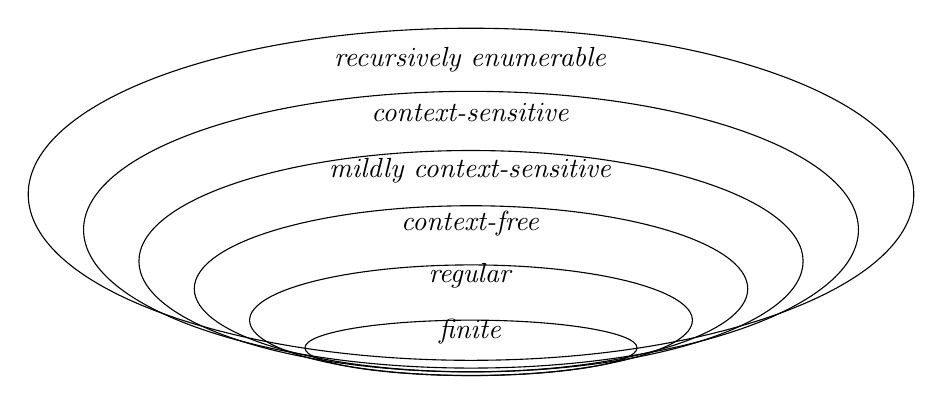
\begin{tikzpicture}          
	\draw (0,-0.65) ellipse (16em and 6em);    
        \draw (0,-1.1) ellipse (14em and 5em);            
        \draw (0,-1.5) ellipse (12em and 4em);            
        \draw (0,-1.85) ellipse (10em and 3em);            
        \draw (0,-2.25) ellipse (8em and 2em);            
        \draw (0,-2.6) ellipse (6em and 1em);
        %
        \node at (0em,3em) {\textit{recursively enumerable}};
        \node at (0em,1.1em) {\textit{context-sensitive}};
        \node at (0em,-1em) {\textit{mildly context-sensitive}};
        \node at (0em,-2.9em) {\textit{context-free}};
        \node at (0em,-4.8em) {\textit{regular}};
        \node at (0em,-6.8em) {\textit{finite}};
\end{tikzpicture}
\caption{The extended Chomsky hierarchy from \citep{JagerRogers12}.}
\label{fig:chomhier}
\end{center}
\end{figure}


This hierarchy represents nested classes of formal languages aligned with respect to their expressive complexity.
On the very top of the hierarchy, there are \textbf{recursively enumerable} languages.
Those are the languages that can be physically computed, i.e.\ realized by a computer in the universe\footnote{The current definition is based on the physical Church-Turing thesis \citep{Church1936,Turing1937a,Turing1937b}.} \citep{Chomsky1956}.
An example of such a language contains all polynomial equations with integer coefficients that have a solution in the integers \citep{Goldberg2018}.
Although such a language exists, there is no method of deterministically predicting if an equation has such a solution.
Below, there are \textbf{context-sensitive} languages that recognize non-linear%
\footnote{The non-linearity refers to the growth of the number of $a$: every following number is \emph{much} larger than the previous.
For example, patterns such as $a^{2n}$, where $n$ is greater than $0$, are non-linear.}
patterns, such as the language of primes \citep{HartmanisShank1968}.
There are subclasses of context-sensitive languages which are a better fit for natural language syntax, such as \textbf{mildly context-sensitive} languages.
They are a good fit for syntactic dependencies as they handle cross-serial dependencies such as some cases of copying; see \citep{Huybregts1984,Joshi1985,Shieber1985,Kallmeyer2010} discussing syntax, and \citep{Culy1985} about a context-sensitive pattern in morphology.
The machine corresponding to \textbf{context-free} languages uses a stack of a potentially infinite size: in such a way, it recognizes patterns such as $a^{n}b^{n}$, \emph{``have as many $a$ as $b$''} \citep{HopcroftEtAl2006}.
\textbf{Regular} languages are limited to the dependencies that can be recognized by an FSA \citep{HopcroftEtAl2006}.
It is commonly assumed that morphology and phonology are regular \citep{Johnson1972,KaplanKay94,BeesleyKartunnen03,RoarkSproat2007}, and I will come back to this topic in the following paragraphs.
Finally, at the very bottom of the hierarchy, one can see a class of \textbf{finite} languages that refer to a finite number of strings.
Classes that are more complex than mildly context-sensitive dependencies are rarely discussed in connection with natural languages: they are too powerful.

Finite-state models correspond to regular languages, and were introduced in $1940$s by \cite{McCullochPitts1943}.
\cite{Chomsky1956}, however, theorized that this type of modeling does not seem to be suitable for natural languages, although in the following years his arguments were shown to be inconclusive, and the question about the regular nature of linguistic dependencies was reopened again.
Also, there was a significant number of applications of finite-state machines to language-related tasks, such as text search \citep{Thompson1968}, machine translation \citep{OncinaEtAl1994,KnightAlOnaizan1998,BangaloreRiccardi2002}, speech recognition \citep{Caseiro2003,MohriPereiraRiley2002,MohriPereiraRiley2008}, semantic parsing \citep{JonesJohnsonGoldwater2011,JonesJohnsonGoldwater2012}, and others.
The restrictiveness of finite-state models is frequently used to balance the robustness of neural networks.
For example, a neural FST-based pronunciation learning model was designed by \cite{Bruguier2017PronunciationLW}.
Additionally, \cite{RoarkEtAl2019} use a neural network guided by a regular grammar to assign pronunciations to words.
At the same time, linguists and computer scientists started to employ regular languages and finite-state models as a tool to research the complexities of patterns in human languages, see \cite{Hulden2014} discussing the main milestones.



The regular nature of phonology was examined several decades ago by \citep{Johnson1972,Kaplan1981PhonologicalRA,KaplanKay94}.
Importantly, \cite{KaplanKay94} show that all SPE-style transformational rules \citep{ChomskyHalle1968}, can be represented as finite-state machines.
Since all attested phonological patterns can be modeled as SPE-style rules, and since SPE-style rules are regular, the complexity of regular languages is a good upper bound for phonological dependencies.
In the same paper, they also presented a set of modeling tools and used them to capture patterns such as nasal assimilation and epenthesis.


\cite{Koskenniemi1983}, and later \cite{BeesleyKartunnen03} show that finite-state machinery is sufficient for encoding morphological dependencies as well.
Even the non-concatenative morphology can be modeled in such a way \citep{Kay1987,Beesley1996,Kiraz1996}.
For more examples of applications of finite-state methods in linguistics, see \citep{GildeaJurafsky1996,RocheSchabes1997,Hetherington2001,JurafskyMartin2009}.
Although regular languages are a good fit for linguistic patterns, research shows that the full power of regular languages is not necessary, and \emph{subregular} languages that are discussed further provide a tighter fit for phonology and morphology.


\subsection{Subregular languages and their linguistic importance}
\label{subgsgf}

The class of regular languages can be subdivided into a nested hierarchy of \emph{subregular} classes --- \textbf{subregular hierarchy}.
``Parent'' classes properly subsume their ``children'' classes, and thus the former are more powerful than the latter.
The ``sibling'' relation implies that the classes are not known to subsume each other.

\begin{figure}[h!]
\begin{center}
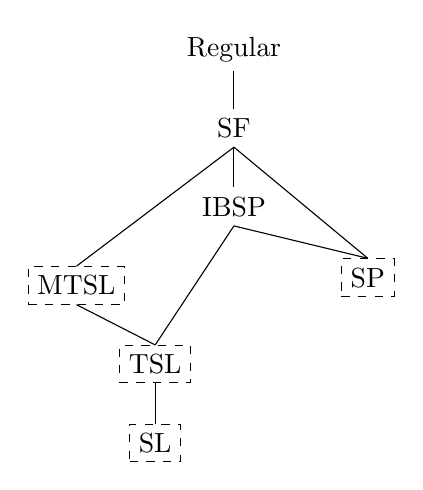
\begin{tikzpicture}[
    highlight/.style = { draw, rectangle, dashed }
    ]
\node (R) at (0,9.5) {Regular};
\node (SF) at (0,8.5) {SF};
\node (IBSP) at (0,7.5) {IBSP};
\node[highlight] (MTSL) at (-2,6.5) {MTSL};
\node[highlight] (TSL) at (-1,5.5) {TSL};
\node[highlight] (SP) at (1.7,6.6) {SP};
\node[highlight] (SL) at (-1,4.5) {SL};
%
\foreach \Source/\Target in {%
        R.south/SF.north,
        SF.south/MTSL.north,
        SF.south/IBSP.north,
        SF.south/SP.north,
        MTSL.south/TSL.north,
        IBSP.south/TSL.north,
        IBSP.south/SP.north,
        TSL.south/SL.north%
    }
\draw (\Source) to (\Target);
\end{tikzpicture}
\caption{Some of the classes of the subregular hierarchy; the subregular classes discussed further in this chapter and in Chapter 3 are boxed.}
\label{subreghier}
\end{center}
\end{figure}

Figure \ref{subreghier} shows some of the subregular classes, namely the ones that are crucially important for modeling linguistic dependencies, and therefore extensively used in this dissertation.
Those are strictly local (SL), strictly piecewise (SP), tier-based strictly local (TSL) and multi-tier strictly local (MTSL) languages.
The crucial difference between these languages is in the types of dependencies they can capture, see Table \ref{subregclasses}.
The combined functionality of those classes covers local dependencies and long-distance dependencies with or without a blocker.


\begin{table}[h!]
\begin{center}
\begin{tabular}{|l|l|}
\hline
\textbf{Language}      & \textbf{Dependencies it can handle}                       \\ \hline
\textit{\textbf{SL}}   & only local dependencies                                   \\ \hline
\textit{\textbf{SP}}   & long-distance dependencies without blocking (any number thereof) \\ \hline
\textit{\textbf{TSL}}  & long-distance dependencies with blocking                  \\ \hline
\textit{\textbf{MTSL}} & multiple long-distance dependencies with blocking         \\ \hline
\end{tabular}
\caption{Types of dependencies captured by some of the subregular classes.}
\label{subregclasses}
\end{center}
\end{table}



Subregular languages are encoded by \emph{subregular grammars}.
These subregular grammars operate by blocking some types of substrings or subsequences in well-formed strings of their languages.
A \textbf{substring} is a consecutive part of the string.
For example, \emph{ab}, \emph{aba}, and \emph{abacd} are substrings of the string \emph{abacd}, whereas \emph{aa} and \emph{bcd} are not, because these symbols are not adjacent in the string \emph{abacd}.
\textbf{Subsequences} can be seen as a non-consecutive counterpart of substrings.
A string $u$ is a subsequence of $w$ if all elements of $u$ can be found in $w$, and the order of those elements is preserved.
Continuing the previous example, both \emph{aa} and \emph{bcd} are indeed subsequences of \emph{abacd}.
Importantly, the elements of substrings and subsequences cannot violate the order in which the elements appeared in the original string: \emph{ca} is neither a substring nor a subsequence of the string \emph{abacd}.
Subregular grammars are always defined for some particular locality, so a $2$-local grammar operates with substrings or subsequences of the length $2$.
Substrings and subsequences will be formally defined in the next two subsections (Definition 2.1.1 in Section \ref{substringformal}, and Definition 2.1.4 in Section \ref{SPformaldef}; see also \citep[a.o.]{ElzingaEtAl2008,Rogers-HeinzEtAl-2010-LPTSS,Fu2011}).

While \emph{positive grammars} list all allowed substructures of their languages, the \emph{negative} ones list the substructures that must not be encountered in well-formed strings of their languages.
Moreover, for the subregular classes discussed in this thesis, these grammars are equivalent: for every negative grammar, it is possible to construct a positive grammar that generates the same language, and vice versa.

The example grammars discussed above are negative grammars, so they prohibit certain substructures in well-formed strings of their languages.
\textbf{Strictly local} (SL) grammars filter strings that violate some local dependency in the string, i.e.\ contain ill-formed \emph{substrings} \citep{Heinz-2010-SEL}.
For example, a language \emph{ab, abab, ababab, etc.} contains any possible string of $a$ and $b$ that does not contain the substrings $aa$ and $bb$.
\textbf{Tier-based strictly local} (TSL) grammars project a potentially smaller string from the input string by using a tier alphabet.
These grammars evaluate the relatively local dependencies among the elements of the \emph{tier alphabet}, whereas all other symbols are ``transparent'' for the grammar \citep{HeinzRawal11}.
For example, if the tier contains $a$ and $b$ and the string is $bccacbc$, the \emph{tier image} of that string is $bab$.
If a TSL constraints are $ba$ or $ab$, the string $bccacbc$ will be ruled out, since its tier image contains the illicit bigrams.
\textbf{Multi-tier strictly local} (MTSL) grammars can have more than just a single tier, and, therefore, multiple tier images are evaluated with respect to multiple local grammars \citep{DeSantoGraf19FG}.
\textbf{Strictly piecewise} (SP) grammars restrict certain \emph{subsequences} in well-formed strings of their languages \citep{Rogers-HeinzEtAl-2010-LPTSS,Heinz10ldp}.
For example, if a subsequence $xx$ is prohibited, a string $xaaax$ is ruled out.
In such a way, SL, SP, TSL and MTSL grammars model a wide range of local and long-distant dependencies \citep{Heinz11part1,HeinzRawal11,Heinz-Lai-2013-VHS,AksenovaEtAl16,ChandleeHeinz2018}.


There are other subregular classes not listed here such as star free (SF), interval-based strictly piecewise (IBSP), input-output tier-based strictly local (IO-TSL) and its subclasses, piecewise testable (PT), etc., but they are out of scope of this dissertation \citep{Lawson2003,Graf18NELS}.
Additionally, I will only discuss grammars working with strings, but this approach is currently extended to other representations as well \citep{chandlee-etal-2019-learning,chandlee-jardine-2019-autosegmental}.

The classes SL, TSL, MTSL, and SP jointly span a wide-ranging array of phonological phenomena.
SL can handle all phenomena that are locally bounded, e.g.\ word-final devoicing or intervocalic voicing.
It can also handle phenomena that are unbounded but proceed in locally bounded steps, for instance some types of vowel harmony where two harmonic vowels are never separated by more than two segments.
Truly unbounded phenomena, on the other hand, require SP, TSL, or MTSL\@.
SP can handle multiple long-distance phenomena at the same time, but only if they do not involve any blocking effects.
An example of that is unbounded tone plateauing, where no low tone may occur within an interval spanned by two high tones, no matter how far apart those two tones are.
For long-distance phenomena with blocking, one has to use TSL, but TSL is not as capable as SP when it comes to enforcing multiple long-distance dependencies in parallel.
This shortcoming is remedied by TSL's extension MTSL\@.
Neither TSL nor MTSL can handle unbounded tone plateauing, though, as will be explained in detail in Sec.~\ref{tslsubsection}.
While, the next few subsections will greatly expand on this overview, it should already be apparent that these subregular classes do indeed cover a lot of empirical ground.

The \textbf{strong subregular hypothesis} interprets the large empirical coverage of these few subclasses as a general indication that natural language phonology and phonotactics are much more restricted than previously believed --- in particular, the class of regular languages is too generous an upper bound and subregular classes provide a better fit for phonology \citep{Heinz10ldp}.
In line with phonotactics, \cite{AksenovaEtAl16} shows that subregular languages are a good fit for morphotactic dependencies.
The well-formedness conditions imposed on languages of generalized and monomorphemic quantifiers are also subregular.
There are likewise applications of subregular grammars to syntax  \citep{Graf17Rutgerstalk,DeSantoGrafDrury2017,VuEtAl19SCiL}.
These findings suggest that subregularity play an important role across many distinct language models, thereby bolstering the strong subregular hypothesis.

In the rest of the chapter, I focus on SL, SP, TSL and MTSL languages and grammars, and provide linguistically-motivated examples of those.
Additionally, I define these classes mathematically and describe the corresponding classes of finite-state automata.
Later, in chapter 3, I will model those and some other dependencies, and show how their subregular grammars can be learned from real data.
Table \ref{fig:subrepattenslfg} summarizes patterns that are discussed further and subregular classes to which they belong.


\begin{table}[h!]
\centering
\begin{tabular}{|>{\centering\arraybackslash}m{0.2\textwidth}|>{\centering\arraybackslash}m{0.2\textwidth}|>{\centering\arraybackslash}m{0.2\textwidth}|>{\centering\arraybackslash}m{0.2\textwidth}|}
\hline
 \centering \textbf{SL} & \centering \textbf{SP}                   & \centering \textbf{TSL} & \textbf{MTSL} \\ \hline
\multicolumn{4}{|c|}{\textit{word-final devoicing and obstruent voicing assimilation}}                                       \\ \hline
                      {\Large\faCheck}        &    \cellcolor{gray!50}\faTimes                           &                             {\Large\faCheck} &          {\Large\faCheck}                     \\ \hline
\multicolumn{4}{|c|}{\textit{unbounded tone plateauing}}                                                                     \\ \hline 
          \cellcolor{gray!50}\faTimes                    &                              {\Large\faCheck} &               \cellcolor{gray!50}\faTimes               &                              \cellcolor{gray!50}\faTimes \\ \hline
\multicolumn{4}{|c|}{\textit{sibilant harmony in voicing and anteriority, no blockers}}       \\ \hline
                  \cellcolor{gray!50}\faTimes            &                              {\Large\faCheck} &                   {\Large\faCheck}           &{\Large\faCheck}                               \\ \hline
\multicolumn{4}{|c|}{\textit{vowel harmony in ATR, nasalized vowels are blockers}}             \\ \hline
                  \cellcolor{gray!50}\faTimes            &                              \cellcolor{gray!50}\faTimes &            {\Large\faCheck}                  &   {\Large\faCheck}                            \\ \hline
\multicolumn{4}{|c|}{\textit{vowel harmony in ATR and rounding, some vowels are blockers for rounding}}             \\ \hline
                  \cellcolor{gray!50}\faTimes            &                              \cellcolor{gray!50}\faTimes &            {\Large\faCheck}                  &   {\Large\faCheck}                            \\ \hline
\multicolumn{4}{|c|}{\textit{sibilant harmony in voicing and anteriority, voiceless obstruents are blockers for voicing}} \\ \hline
                      \cellcolor{gray!50}\faTimes        &                              \cellcolor{gray!50}\faTimes &              \cellcolor{gray!50}\faTimes                &  {\Large\faCheck}  \\ \hline
\end{tabular}
\caption{Subregular patterns attested in natural languages and discussed in sections 2.1.3-6.}
\label{fig:subrepattenslfg}
\end{table}



\subsection{Local restrictions as SL languages}
\label{russianwfdpatternn}

The subregular class of strictly local (SL) languages captures local dependencies, and many restrictions in phonology have a purely local nature \citep{RogersPullum2011}.
Indeed, most of the patterns of phonological assimilation affect adjacent segments.
In what follows, I exemplify SL languages using several purely local phenomena, and then formally introduce them using the notion of $k$-factor and the property of suffix substitution closure \citep{RogersEtAl13}.

\subsubsection{Intuitive definition}

In what follows, the SL languages are demonstrated through two local phenomena happening in Russian: one of them prohibits voiced obstruents in the word-final position, and another one enforces adjacent obstruents to agree in voicing.
Additionally, I show the interaction between these two patterns.

\paragraph{Russian obstruent assimilation and word-final devoicing}
The examples (1-2) below show that the consonant of the preposition \emph{iz} `from' agrees in voicing with the obstruent of the following word.%
\footnote{I do not discuss exceptions to this rule, such as the well-formedness of the cluster [sv].}

\medskip
\begin{tabular}{lll}
(1) & i[z B]erlina & `from Berlin' \\
(2) & i[s P]ragi & `from Prague'
\end{tabular}
\medskip

Additionally, in Russian, as well as in other languages such as German, there is a word-final devoicing that prohibits the appearance of a voiced obstruent in a word-final position \citep{Wiebke1995,Padgett2002ms}.
For example, \emph{lug} `field' is realized as \emph{lu[k]}.
In this case, the same cluster of obstruents might appear voiceless word-finally, and voiced in other positions of the word, see the pairs of examples in (3-4) and (5-6).

\medskip
\begin{tabular}{lllclll}
(3) & mo[sk] & `brain' & $\sim$ & (4) & mo[zg]i & `brains' \\
(5) & dro[st] & `thrush' & $\sim$ & (6) & dro[zd]y & `thrushes'
\end{tabular}
\medskip

These two generalizations can be captured in a \emph{strictly local} way, namely, by prohibiting illicit substrings.
Assume that the inventory of obstruents is $\{z, s, b, p, g, k\}$, where $z$, $b$, and $g$ are voiced, and $s$, $p$ and $k$ are voiceless.
It is never possible to see two (or more) disagreeing obstruents adjacent to each other, i.e.\ the target SL grammar needs to prohibit $zs$, $zp$, $zk$, $sz$, $sb$, $sg$, etc.


To target voiced obstruents at the end of the word, the grammar needs to be able to differentiate between the word-final and other positions.
For this reason, strings are usually annotated with the markers \bow\ and \eow\ denoting the beginning and the end of the string \citep{RogersPullum2011}.
Then, the SL grammar capturing word-final devoicing needs to rule out $z\eow$,  $g\eow$, and $b\eow$.

\begin{figure}[h!]
\begin{center}
\begin{tikzpicture}%[baseline]
\node (1) at (0,0) {$\rtimes$};
\node (2) at (0.5,0) {m};
\node (3) at (1,0) {o};
\node (4) at (1.5,0) {s};
\node (5) at (2,0.05) {k};
\node (6) at (2.5,0) {$\ltimes$};
%\node (1) at (0,0) {$\rtimes$};
%\node[at=(1.base)] (2) {m};
%\node[at=(2.base)] (3) {o};
%\node[at=(3.base)] (4) {s};
%\node[at=(4.base)] (5) {k};
%\node[at=(5.base)] (6) {$\ltimes$};
\end{tikzpicture}
\hspace{2em}
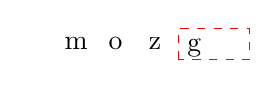
\begin{tikzpicture}
\node (1) at (0,0) {$\rtimes$};
\node (2) at (0.5,0) {m};
\node (3) at (1,0) {o};
\node (4) at (1.5,0) {z};
\node (5) at (2,-0.05) {g};
\node (6) at (2.5,0) {$\ltimes$};
\draw [dashed, red] (1.8, -0.2) -- (1.8, 0.2) -- (2.7, 0.2) -- (2.7, -0.2) -- (1.8, -0.2);
\end{tikzpicture}
\vspace{1em}

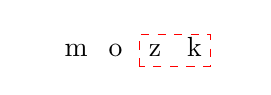
\begin{tikzpicture}
\node (1) at (0,0) {$\rtimes$};
\node (2) at (0.5,0) {m};
\node (3) at (1,0) {o};
\node (4) at (1.5,0) {z};
\node (5) at (2,0.05) {k};
\node (6) at (2.5,0) {$\ltimes$};
\draw [dashed, red] (1.3, -0.2) -- (1.3, 0.2) -- (2.2, 0.2) -- (2.2, -0.2) -- (1.3, -0.2);
\end{tikzpicture}
\hspace{2em}
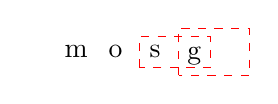
\begin{tikzpicture}
\node (1) at (0,0) {$\rtimes$};
\node (2) at (0.5,0) {m};
\node (3) at (1,0) {o};
\node (4) at (1.5,0) {s};
\node (5) at (2,-0.05) {g};
\node (6) at (2.5,0) {$\ltimes$};
\draw [dashed, red] (1.3, -0.2) -- (1.3, 0.2) -- (2.2, 0.2) -- (2.2, -0.2) -- (1.3, -0.2);
\draw [dashed, red] (1.8, -0.3) -- (1.8, 0.3) -- (2.7, 0.3) -- (2.7, -0.3) -- (1.8, -0.3);
\end{tikzpicture}
\end{center}
\caption{Evaluation of strings \emph{mozg}, \emph{mozk}, \emph{mosg} and \emph{mosk} by an SL grammar capturing obstruent cluster assimilation and word-final devoicing.}
\label{mozgi}
\end{figure}

Figure \ref{mozgi} shows how the SL grammar outlined above evaluates the pronunciations \emph{mozg}, \emph{mozk}, \emph{mosg} and \emph{mosk}.
The string \emph{mozg} has its obstruents agree in voicing, but the final obstruent is voiced, and therefore ruled out by the restriction $g\eow$.
The final obstruent in \emph{mozk} is voiceless, but now the cluster disagrees and therefore ruled out by $zk$.
In \emph{mosg}, both violations are present.
Finally, the form \emph{mosk} contains no violations, and indeed, this is the correct pronunciation of the corresponding Russian word.

The illicit substrings such as $g\eow$ and $zk$ are the \emph{restrictions} defined by the grammar.
A set of restrictions $R$ of a negative grammar lists all substrings that \emph{cannot} be found in well-formed strings of the language.
An \emph{alphabet} of the language, usually denoted as $\Sigma$, includes the list of symbols the language uses.
In this case, $\Sigma$ includes all Russian phonemes.
Finally, every grammar defines its \emph{locality}, namely, the size of the longest string prohibited by that grammar; it is usually referred to as $k$ \citep{McNaughtonPapert1971,RogersPullum2011}.
In the case of the SL grammar capturing Russian well-formedness conditions, all the prohibited strings are of length $2$ ($k=2$); such substrings are also called \emph{bigrams} or \emph{$2$-factors}.
The Russian SL grammar is then strictly $2$-local, or SL-$2$.
These three components -- the alphabet $\Sigma$, the set of restriction $R$, and the locality window $k$ -- define SL grammars, see Grammar \ref{slwfdocass55}.

{
\renewcommand{\tablename}{Grammar}
\begin{table}[h!]
\begin{center}
\begin{tabular}{rl}
\textit{SL grammar}  & Russian obstruent voicing assimilation and word-final devoicing \\
\textit{$\Sigma$ =}      &  \{a, b, v, g, d $\dots$ z, s, p, k $\dots$ \textepsilon, $^j$u, $^j$a\}   \\
\textit{$R$ =} & $\langle$zs, zp, zk, sz, sb, sg $\dots$ z\eow,  g\eow, b\eow, d\eow $\rangle$  \\
\textit{$k$ =}      & $2$          
\end{tabular}
\caption{SL-$2$ grammar for Russian obstruent voicing assimilation and word-final devoicing.}
\label{slwfdocass55}
\end{center}
\end{table}
}

SL grammars disallow the appearance of the banned clusters such as $gs$ or $zk$, however, they do not induce the change of the ill-formed segments.
The perspective of changing one form into another is examined in the Section 2.2 discussing modeling transformations.
SL models are useful in modeling the well-formedness conditions arising from word-final devoicing, intervocalic voicing, consonant cluster assimilation, and other local phenomena.
However, SL models cannot model long-distance dependencies.

\paragraph{Tuareg sibilant harmony}
Long-distance dependency affects segments that can be located far from each other.
For instance, in Tuareg (Berber), sibilants regressively agree in voicing and anteriority \citep{Hansson2010ber}.
In the examples below, a causative prefix agrees with the sibilant in the root (8-11) but is realized as \emph{s-} if no other sibilant is present (7).
This is an instance of long-distance agreement, and therefore it can happen across an arbitrary number of intervening elements.

\medskip
\begin{tabular}{lll}
(7) & s-\textschwa lm\textschwa d & `\textsc{caus}-learn' \\
(8) & s-\textschwa q:us\textschwa t & `\textsc{caus}-inherit' \\
(9) & z-\textschwa nt\textschwa z & `\textsc{caus}-extract' \\
(10) & \textesh-\textschwa m:\textschwa\textesh\textschwa n & `\textsc{caus}-be.overwhelmed' \\
(11) & \textyogh-\textschwa k:u\textyogh\textschwa t & `\textsc{caus}-saw'
\end{tabular}
\medskip

SL grammars capture only local generalizations, but, for example, in (9), there are $4$ elements separating the agreeing sibilants.
It would imply that the required locality of the SL grammar is at least $6$ to accommodate the two sibilants and everything in-between them.
However, this would not be enough for other cases since there is no upper bound on the number of the intervening segments in-between two agreeing sibilants.
As a result, the power of SL grammars is not enough to capture patterns such as Tuareg sibilant harmony.

Playing devil's advocate, though, one may object that in practice there is such a thing as a longest word due a variety of reasons, e.g.\ performance limitations or limited morphological productivity.
If the longest word has at most $n$ segments, then no phonological phenomenon can involve more than $n$ segments, making in SL-$n$.
But there are multiple problems with this position.
First of all, it ignores the widely assumed distinction between competence and performance.
Second, it assumes that phonology is limited to a single phonological word, which isn't the case either.
At least some phenomena apply across phonological word boundaries, so it is not enough to assume a fixed upper bound on the length of phonological words --- one has to assume a fixed upper bound on the length of phonological dependencies.
Finally, and most importantly, this position ignores succinctness.
The number of possible $n$-grams grows exponentially with $n$: assuming an inventory of 10 distinct sounds, there are $10^2 = 100$ distinct bigrams, $10^3 = 1,000$ trigrams, $10^4 = 10,000$ $4$-grams, and so on.
The size of an SL grammar explodes as we extend to handle increasingly non-local phenomena.
And this also poses a challenge for learnability because larger SL-grammars require more evidence to infer from the training data (a space of $100$ options is more easily explored than one of $10,000$ options).
So even if long-distance phenomena might indeed be limited to some fixed upper bound, this bound is so high for natural languages that an SL grammar simply cannot describe these long-distance phenomena in a succinct and elegant manner that supports efficient learning.


\subsubsection{Formal definition}
\label{substringformal}

SL grammars define languages by listing substrings that cannot appear in well-formed words of those languages.
These substrings are often referred to as $k$-factors, in order to be distinguished from the more NLP-oriented use of the term $n$-gram, that frequently implies the use of probabilistic models \citep{RogersPullum2011,RogersEtAl13}.
Further in this section, I follow \cite{DeSantoGraf19FG} in their algebraic definition of this class.

While $\Sigma$, as previously in this section, denotes the alphabet, $\Sigma^{k}$ is a $k$-long word that uses symbols of that alphabet.
$\Sigma^{*}$ generalizes $\Sigma^{k}$, it employs the \emph{Kleene star} \citep{Kleene1956} to define a word of any length, including length $0$, i.e.\ the empty string $\varepsilon$.
A length of the string $w$ is denoted as $|w|$.

\begin{definition}[\textbf{$k$-factors}]
A string $u$ is a $k$-\emph{factor}, or a \emph{substring} of a string $w$ iff $\exists x, y \in \Sigma^*$ such that $w=xuy$ and $|u| = k$. 
The function $F_k$ maps words to the set of $k$-factors within them:
$$
F_k(w) = \{ u : u \textit{ is a $k$-factor of } w \textit{ if } |w| \geq k, 
\textit{ else } u = w\}
$$
\end{definition}

For example, the $2$-factors of the word $abc$ are $\{ab, bc\}$.
Strictly $k$-local grammars list the $k$-factors that cannot be used in the well-formed strings of their languages, i.e.\ they can be viewed as collections of illicit $k$-factors.
Markers $\bow\not\in\Sigma$ and $\eow\not\in\Sigma$ are used in the same way as previously in Section \ref{russianwfdpatternn}: they are edge markers marking the beginning and the end of the string.


\begin{definition}[\textbf{SL languages and grammars}]
A language $L$ is \emph{strictly $k$-local} (SL$_k$) iff there exists a finite set $S \subseteq F_k (\rtimes^{k-1} \Sigma^* \ltimes^{k-1})$ such that
\[
L = \{ w \in \Sigma^*: F_k(\rtimes^{k-1} w \ltimes^{k-1}) \cap S = \emptyset \}.
\]
We call $S$ a strictly $k$-local grammar, and use $L(S)$  to indicate the language recognized by $S$.
A language $L$ is strictly local iff it is SL$_k$ for some $k \in \mathbb{N}$.
\end{definition}

Consider a language described by a regular expression $(ab)^{*}$.
Its language includes strings such as $\varepsilon$, $ab$, $abab$, $ababab$, etc.
A negative SL-$2$ grammar that describes this language is $S = \{\bow b, a\eow, aa, bb\}$.
Indeed, the well-formed strings of that language cannot start with $b$, end with $a$, and have two $a$ or two $b$ adjacent to each other.
Importantly, a language is strictly $k$-local if it satisfies $k$-local \emph{suffix substitution closure} \citep{RogersPullum2011}.

\begin{definition}[\textbf{Suffix substitution closure}]
\label{suffsubclosure}
For any $k \geq 1$, a language $L$ satisfies  $k$-local suffix substitution closure iff for all strings $u_1, v_1, u_2, v_2$, for any string $x$ of length $k - 1$ if both $u_1 \cdot x \cdot v_1 \in L$ and $u_2 \cdot x \cdot v_2 \in L$, then $u_1 \cdot x \cdot v_2 \in L$.
\end{definition}

For instance, a language $(ab)^*$ is SL-$2$, and it satisfies suffix substitution closure.
Both strings \emph{\textbf{a}b} and \emph{ab\textbf{a}bab} contain the $1$-local substring $a$, and it correctly predicts that the string \emph{ab\textbf{a}b} is also in the language.
However, a language $a^*ba^*$ is not SL.
It is not SL-$2$ since the closure of the strings \emph{\textbf{a}ba} and  \emph{b\textbf{a}a} contains \emph{b\textbf{a}ba}, and it is not in the language.
It is not SL-$3$, because the closure of \emph{\textbf{aa}ba} and \emph{b\textbf{aa}a} contains the illicit form \emph{b\textbf{aa}ba}; and so on.
The language $a^*ba^*$ is not closed under the suffix substitution, and therefore it is not SL.

Apart from the algebraic perspective, strictly local languages can be characterized in automata-theoretic terms.
\cite{RogersPullum2011} describe SL languages as those that can be recognized by FSAs scanning a $k$-symbol window across the input string, and failing on strings that contain factors prohibited by the corresponding grammar.
In such an SL-$k$ automaton, states represent the $k-1$-local suffix of the input string read immediately before now, and the transitions from the states encode symbols that can follow.
If a transition cannot be taken, or if the final activated state is not accepting, the input string is rejected.
When a string is well-formed, there is a part through the automaton that starts in the initial state and ends in the final one.



States of SL-automata encode the previous substring of the input string.
So, for example, in SL-$2$ automaton the states differentiate depending on the symbol that was observed 


\subsection{Long distance restrictions as SP languages}
\label{SPldrestrictions}


While SL grammars can only capture local dependencies, strictly piecewise (SP) grammars generalize exclusively long-distance patterns: %
%Previously, I showed that there is no upper bound on the amount of material in-between two agreeing sibilants, and therefore such generalization cannot be captured locally.
SL grammars prohibit sequences of adjacent segments within words, while SP grammars do not have the requirement of adjacency.
An SP restriction prohibits a certain \emph{order} of elements \citep{Rogers-HeinzEtAl-2010-LPTSS,Fu2011}. 
While an SL restriction $VV$ prohibits two vowels adjacent to each other thus avoiding hiatus, the same SP restriction means that nowhere in the string can there be a vowel followed by another vowel.
The language of such an SP grammar would only include words with no more than a single $V$.


\subsubsection{Intuitive definition}

In this section, I demonstrate how SP grammars can capture patterns of sibilant harmony and unbounded tone plateauing.
SP grammars encode restrictions on the order of elements, and thus cannot differentiate between disharmonic stems and grammatical words exhibiting a blocking effect.





\paragraph{Tuareg sibilant harmony}
Coming back to the pattern of Tuareg sibilant harmony exemplified before in (7-11), it can be modeled with an SP grammar by prohibiting subsequences of disagreeing sibilants.
The bigrams $sz$ and \textesh\textyogh~ are prohibited because their elements disagree in voicing, \textesh$s$ and $z$\textyogh~ disagree in anteriority, etc.
In total, this grammar contains $12$ restrictions $R$ that are listed in Grammar \ref{tuaregsibilanthupd}.

{
\renewcommand{\tablename}{Grammar}
\begin{table}[h!]
\begin{center}
\begin{tabular}{rl}
\textit{SP grammar}  & Tuareg sibilant harmony in voicing and anteriority \\
\textit{$\Sigma$ =}      &  \{s, \textyogh, z, \textesh, \textschwa, d, l, m, t $\dots$\}   \\
\textit{$R$ =} & $\langle$sz, s\textesh, s\textyogh, zs, \textesh s, \textyogh s, z\textesh, z\textyogh, \textesh s, z\textesh, z\textyogh, \textesh z, \textesh z, \textesh\textyogh, \textesh z$\rangle$  \\
\textit{$k$ =}      & $2$          
\end{tabular}
\caption{SP-$2$ grammar for Tuareg sibilant harmony in voicing and anteriority.}
\label{tuaregsibilanthupd}
\end{center}
\end{table}
}

Such an SP grammar has an alphabet that includes all Tuareg phonemes, and its list of restrictions includes all pairs of sibilants disagreeing in voicing or anteriority.
The locality of such grammar is $2$.
Figure \ref{tuaregsthfg} shows that there are no violations in the word \emph{z\textschwa nt\textschwa z}: indeed, no substructure of that string is prohibited.
However, the word \emph{z\textschwa nt\textschwa \textyogh} is ruled out because the subsequence $z$\textyogh~ is ill-formed.


\begin{figure}[h!]
\begin{center}
\begin{tikzpicture}
\node (2) at (0.5,0.57) {z};
\node (3) at (1,0.57) {\textschwa};
\node (4) at (1.5,0.57) {n};
\node (5) at (2,0.57) {t};
\node (6) at (2.5,0.57) {\textschwa};
\node (7) at (3,0.57) {z};
\node (8) at (3,0) {\textcolor{white}{t}};
\end{tikzpicture}
\hspace{3em}
\begin{tikzpicture}
\node (2) at (0.5,0) {\textcolor{red!75!black}{z}};
\node (3) at (1,0) {\textschwa};
\node (4) at (1.5,0) {n};
\node (5) at (2,0) {t};
\node (6) at (2.5,0) {\textschwa};
\node (7) at (3,0) {\textcolor{red!75!black}{\textyogh}};
\path[->, red] (2) edge[bend right = 45] (7);
\end{tikzpicture}
\end{center}
\caption{Evaluation of strings \emph{z\textschwa nt\textschwa z} and \emph{z\textschwa nt\textschwa\textyogh} by an SP grammar capturing sibilant harmony in voicing and anteriority.}
\label{tuaregsthfg}
\end{figure}




\paragraph{Imdlawn Tashlhiyt sibilant harmony}

Now, consider a language closely related to Tuareg, namely, Imdlawn Tashlhiyt (Berber), in which affixal sibilants also regressively harmonize with the stem in voicing and anteriority \citep{Hansson2010ber,McMullin2016}.
The difference is that in Imdlawn Tashlhiyt, the spreading of the voicing feature can be blocked by any intervening voiceless obstruent.
At the same time, similarly to Tuareg, the anteriority harmony exhibits no blocking effect.
Consider the data from \citep{Elmedlaoui1995,Hansson2010} in (12-18), where the causative prefix \emph{s-} illustrates the harmonic pattern.

\medskip
\begin{tabular}{lll}
(12) & s:-uga & `\textsc{caus}-evacuate' \\
(13) & s-as:twa & `\textsc{caus}-settle' \\
(14) & \textesh-fia\textesh r & `\textsc{caus}-be.full.of.straw' \\
(15) & z-bruz:a & `\textsc{caus}-crumble' \\
(16) & \textyogh-m:\textyogh dawl & `\textsc{caus}-stumble' \\
(17) & s-m\textchi azaj & `\textsc{caus}-loathe.each.other' \\
(18) & \textesh-qu\textyogh:i & `\textsc{caus}-be.dislocated'
\end{tabular}
\bigskip

In (12), there are no sibilants in the root, so the prefix is realized as \emph{s-}.
Examples (13-16) show that as previously, the causative affix agrees with the stem sibilant in voicing and anteriority.
However, the voicing harmony can be blocked, and it is exemplified in (17) and (18).
In (17), the sibilants are both anterior, but \textchi~ is stopping the regressive spreading of [+voice], so the prefix is realized as voiceless.
Similarly, in (18), both sibilants are non-anterior, but the voicing spreading is also blocked, this time by $q$. 

In Imdlawn Tashlhiyt, voiceless obstruents are \emph{blockers} for the voicing harmony, and this prevents SP grammars from being able to model the generalization.
The rules of the harmony are the same as before, therefore all restrictions discussed earlier in Grammar \ref{tuaregsthfg} are still valid.
However, there is no way to express a blocking effect in an SP grammar.
An SP restriction is a restriction on the precedence of one segment by another, and therefore the presence of the bigram $sz$ is necessary to rule out disharmonic words such as \emph{saz:twa}.
But the same restriction will necessarily rule out grammatical words such as \emph{sm\textchi azaj}: it will simply ``miss'' the blocker, see Figure \ref{imdlawnbadsp}.


\begin{figure}[h!]
\begin{center}
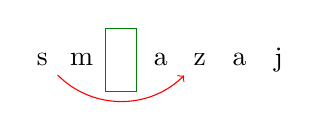
\begin{tikzpicture}
\node (2) at (0.5,0) {s};
\node (3) at (1,0) {m};
\node (4) at (1.5,0) {\textchi};
\node (5) at (2,0) {a};
\node (6) at (2.5,0) {z};
\node (7) at (3,0) {a};
\node (8) at (3.5,0) {j};
\path[->, red] (2) edge[bend right = 45] (6);
\draw[green!50!black] (1.3, -0.4) rectangle (1.7, 0.4);
\end{tikzpicture}
\end{center}
\caption{SP grammar incorrectly rules out Imdlawn Tashlhiyt word \emph{sm\textchi azaj}.}
\label{imdlawnbadsp}
\end{figure}

Increasing the size of the substrings to $3$ will not solve the problem with the blocking effect either.
An SP grammar that finds the word \emph{sm\textchi azaj} correct will inevitably accept all subsequences of that word.
As a result, it would incorrectly predict the well-formedness of the word \emph{smzaj}, where $s$ and $z$ disagree in voicing without the presence of a blocker.



\paragraph{Unbounded tone plateauing}
The ability of SP grammars to see substructures independently of other elements of the string gives them the power to encode \emph{unbounded tone plateauing} (UTP), as attested in Luganda (Niger-Congo).
In that language, low tones are realized as high if they are surrounded by high tones \citep{HymanKatamba2010}.
This makes it impossible for a well-formed word in Luganda to have low tones surrounded by high tones, see the data in (19) cited by \citep{Hyman2011,Jardine2016}.
Accented vowels indicate high tones, and other vowels are low.

\medskip
\begin{tabular}{llcl}
(19) & bik\'opo byaa-wal\'usiimbi & $\rightarrow$ & bik\'op\'o by\'a\'a-w\'al\'usiimbi \\
& `the cups of Walusimbi' &&
\end{tabular}
\medskip

Using the letters $H$ and $L$ to indicate high and low tones, we can express the generalization as ``never have one or more L in-between two H''.
This allows for strings such as \emph{HHL} and \emph{LLLHHHL}, but prohibits ones such as \emph{HHLLLHH}.
Due to the long-distant nature of SP grammars, a $3$-local SP grammar can capture UTP by ruling out words that contain a subsequence $HLH$, see Figure \ref{imdlawngoodsp}.

\begin{figure}[h!]
\begin{center}
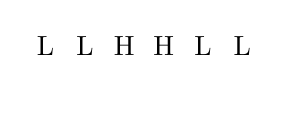
\begin{tikzpicture}
\node (1) at (0,0) {L};
\node (2) at (0.5,0) {L};
\node (3) at (1,0) {H};
\node (4) at (1.5,0) {H};
\node (5) at (2,0) {L};
\node (6) at (2.5,0) {L};
\node (6) at (2.5,-0.3) {\textcolor{white}{L}};
\end{tikzpicture}
\hspace{3em}
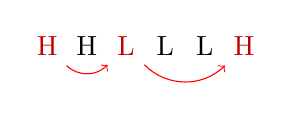
\begin{tikzpicture}
\node (1) at (0,0) {\textcolor{red!75!black}{H}};
\node (2) at (0.5,0) {H};
\node (3) at (1,0) {\textcolor{red!75!black}{L}};
\node (4) at (1.5,0) {L};
\node (5) at (2,0) {L};
\node (6) at (2.5,0) {\textcolor{red!75!black}{H}};
\path[->, red] (1) edge[bend right = 45] (3);
\path[->, red] (3) edge[bend right = 45] (6);
\end{tikzpicture}
\end{center}
\caption{SP grammar captures the UTP pattern.}
\label{imdlawngoodsp}
\end{figure}

{
\renewcommand{\tablename}{Grammar}
\begin{table}[h!]
\begin{center}
\begin{tabular}{rl}
\textit{SP grammar}  & Luganda unbounded tone plateauing \\
\textit{$\Sigma$ =}      &  \{H, L\}   \\
\textit{$R$ =} & $\langle$HLH$\rangle$  \\
\textit{$k$ =}      & $3$          
\end{tabular}
\caption{SP-$3$ grammar for Luganda unbounded tone plateauing.}
\label{utpsuccessfulsp}
\end{center}
\end{table}
}

Strictly piecewise grammars capture one or more long-distance phenomena that do not exhibit blocking effects.
They prohibit subsequences of strings, therefore ruling out all words that contain the illicit substructure.
For example, the restriction $zs$ means that nowhere in the string, $z$ can be followed by $s$.
However, blocking effects cannot be captured via an SP grammar, because the grammar is not sensitive to the presence of the blockers that make the banned substructure acceptable.
A pattern where a substring $s\dots z$ is prohibited, but $s\dots k \dots z$ is allowed is not SP: ruling out the former one would rule out the latter one as well.
Blockers do not change the presence of an illicit subsequence.
Purely short-distant restrictions such as the word-final devoicing also cannot be expressed by an SP grammar: the restriction $b\eow$ prohibits \emph{any} string containing $b$, because $\eow$ always follows $b$ in a word annotated with the word-final marker $\eow$.





\subsubsection{Formal definition}
\label{SPformaldef}

An SP grammar is defined as a list of subsequences prohibited in well-formed strings of its language.
Further, I define the notion of the subsequence and the SP languages formally following \cite{Rogers-HeinzEtAl-2010-LPTSS}, and then provide an alternative definition in automata-theoretic terms.



\begin{definition}[\textbf{Subsequences}]
A string $v$ is a subsequence of $w$, $v \sqsubseteq~ w$, if $v$ is an empty string, or if $v = \sigma_1\sigma_2\dots\sigma_n$, and there is a collection of substrings $x_1, \dots, w_n \in \Sigma^*$, such that those substrings can be placed between the elements of $v$ thus obtaining $w = w_0\sigma_1 w_1\dots\sigma_n w_n$.

Then all $k$-long subsequences $P_k(w)$ of a word $w \in \Sigma^*$ can be computed as

$$ P_{k}(w) = \{v \in \Sigma^{k} : v \sqsubseteq w\} $$

Similarly, $P_{\leq k}(w)$ lists all subsequences of $w \in \Sigma^*$  of the length up to $k$.

$$ P_{\leq k}(w) = \{v \in \Sigma^{\leq k} : v \sqsubseteq w\} $$
\end{definition}



For example, consider a string $w = abcd$.
Then $P_{3}(w) = \{abc, abd, acd\}$, and $P_{\leq 3}(w) = P_{3}(w) \cup \{\varepsilon, a, b, c, d, ab, ac, ad, bc, bd, cd\}$, where $\varepsilon$ is the empty string.

\begin{definition}[\textbf{SP languages and grammars}]
A language is SP-$k$ if there exists a set of subsequences $S \subseteq \Sigma^k$ such that

\[
	L(\mathcal{G}) = \{w \in \Sigma^* : P_{\leq k}(w) \subseteq P_{\leq k}(S)\}.
\]
\end{definition}


The exact reason why SP grammars cannot capture the blocking effect is their \emph{closure under subsequence}; see \citep{Rogers-HeinzEtAl-2010-LPTSS} for other properties of SP languages and grammars.

\begin{definition}[\textbf{Subsequence closure}]
Given a word $w \in L$, all strings $v$ that are subsequences of $w$, $v \sqsubseteq w$, also belong to the language $L$.
\end{definition}


Alternatively, an SP language can be defined as a deterministic finite automaton (DFA) of a particular shape.
Such a machine is a quintuple $\mathcal{M} = \langle Q, \Sigma, q_0, \delta, F\rangle$, where $Q$ is a finite set of states, $\Sigma$ is the alphabet, $q_0$ is the unique initial state, $\delta$ is the transition function, and $F$ is the set of accepting states.
The following properties are true for the automata recognizing SP languages.
All states of $\mathcal{M}$ are accepting, i.e.\ $F = Q$.
If $q_2$ is reachable from $q_1$ and if there is no transition reading $\sigma \in \Sigma$ from $q_1$, there will be no transition reading $\sigma$ from $q_2$ (missing edges propagate down).
All cycles are self-edges.
If such a machine accepts a string $w\cdot v\cdot u : w, v, u \in \Sigma^{*}$, it necessarily accepts a string $w\cdot u$.
This dependency, however, is not true in the other direction: if such a DFA accepts $w\cdot u$, there could be $v \in \Sigma^*$ such that $w\cdot v\cdot u$ is not an acceptable input sequence.
A DFA with these properties accepts only SP languages.







\subsection{Long-distant dependencies with blocking as TSL languages}
\label{tslsubsection}


Earlier, I showed that SL and SP grammars cannot capture long-distance harmonies with a blocking effect.
SL grammars can only express local generalizations, and SP restrictions target certain subsequences and therefore are not sensitive to the presence of blockers.
Tier-based strictly local (TSL) grammars capture long-distance dependencies by \emph{making them local} over the tier \citep{HeinzRawal11}.

\subsubsection{Intuitive definition}

I demonstrate the capacities of TSL grammars using the examples of vowel harmony in Karaj\'a (ATR harmony with nasalized blockers) and Buryat (ATR and rounding harmony without blockers).

\paragraph{Karaj\'a vowel harmony}

Consider vowel harmony in Karaj\'a (Macro-J\^e), where a tense vowel spreads the advanced tongue root (ATR) feature leftwards.
It makes it impossible to have a lax vowel followed by a tense one.
This spreading can be blocked by intervening nasalized vowels; they are opaque for this harmony \citep{Ribeiro2002}.
\bigskip

\begin{tabular}{llll}
(20) & woku & {[}woku{]} & `inside' \\
(21) & d\textopeno r\textepsilon & {[}d\textopeno r\textepsilon{]} & `parrot' \\
(22) & bu\texthtd\textepsilon & {[}bu\texthtd\textepsilon{]} & `little, few' \\
(23) & br\textopeno r\textepsilon d$\breve{\imath}$ & {[}broren$\breve{\imath}${]} & `cow (\emph{lit.} deer-similar.to)' \\
(24) & d\textopeno r\textepsilon~ de & {[}dorede{]} & `parrot's wing' \\
(25) & rak\textopeno h\textopeno\texthtd\textepsilon k\~ore & {[}rak\textopeno h\textopeno\texthtd\textepsilon k\~ore{]} & `He/she didn't hit it.' \\
(26) & r\textepsilon b\~\textschwa re & {[}r\textepsilon m\~\textschwa re{]} & `I caught (it).'
\end{tabular}

\bigskip
The data in (20-26) exemplifies the rule of harmony and is discussed in more detail in \cite{Ribeiro2002}.
Note, that the harmony is reflected in the transcriptions and not in the orthography of the language.
Stems in Karaj\'a can contain tense (20) or lax (21) vowels, and the lax vowels can only follow the tense ones (22).
A tense vowel starts its harmonic domain and spreads the [+ATR] feature regressively (23-24).
However, nasalized vowels such as \emph{\~o} and \~\textschwa~ are opaque for this spreading: they do not enforce the agreement of the vowel thus allowing lax vowels to precede the nasal ones, even if a tense vowel follows it (25-26).

A TSL grammar is defined for a \emph{tier alphabet} $T$ that includes all segments that are relevant for the long-distance dependency.
All vowels are relevant for the harmony, i.e.\ they are either undergoers (lax vowels), or blockers (nasalized vowels), or start the harmonic domain (tense vowels).
Therefore in this case, the tier alphabet contains all vowels, $T = \{$\textepsilon$, o, e, u,$ \textopeno, \emph{\~o}, \~\textschwa~$, a, \dots\}$.
A \emph{tier image} of the string is a representation of that string where only the elements of $T$ are preserved.
For example, the tier image of \emph{rak\textopeno h\textopeno\texthtd\textepsilon k\~ore} is \emph{a\textopeno\textopeno\textepsilon\~oe}.
Finally, the set of restrictions $R$ is defined for the tier representations of the string.
In other words, the prohibited elements are the substrings that must not be observed in the tier representations of well-formed words of the language.

To construct the tier grammar for the Karaj\'a vowel harmony, one needs to prohibit all combinations of a lax vowel followed by a tense one, i.e.\ \textepsilon$e,$ \textepsilon$o,$ \textopeno$o,$ \textopeno$u$, etc.
The presence of the nasalized vowels on the tier allows for sequences such as \textepsilon$\dots$\~\textschwa$\dots e$, where the opaque element blocks spreading of the ATR feature.
Indeed, in such cases, the lax vowel \textepsilon~ and the tense  $e$ are not tier adjacent because of the intervening \~\textschwa.
This makes TSL grammars a good fit for many harmonic patterns, even if they exhibit blocking effects.

{
\renewcommand{\tablename}{Grammar}
\begin{table}[h!]
\begin{center}
\begin{tabular}{rl}
\textit{TSL grammar}  & Karaj\'a vowel harmony in ATR \\
\textit{$\Sigma$ =}      &  \{\textepsilon, \~o, \~\textschwa, o, e, u, \textopeno, a, \~\textschwa, \~a, \~o $\dots$ b, \texthtd, d, r $\dots$\} \\
\textit{$T$ =}      &  \{\textepsilon, \~o, \~\textschwa, o, e, u, \textopeno, a, \~\textschwa, \~a, \~o $\dots$\}  \\
\textit{$R$ =} & $\langle$\textepsilon e, \textepsilon o,  \textopeno o, \textopeno u, \textepsilon u $\dots\rangle$  \\
\textit{$k$ =}      & $2$          
\end{tabular}
\caption{TSL-$2$ grammar for Karaj\'a vowel harmony in ATR.}
\label{fdfsdrgr}
\end{center}
\end{table}
}


\begin{figure}[h]
\hspace{0.5em}
\begin{tikzpicture}
\node (0) at (0,0) {\bow};
\node (1) at (0.5,0) {b};
\node (2) at (1,0) {u};
\node (3) at (1.5,0) {\texthtd};
\node (4) at (2,0) {\textepsilon};
\node (5) at (2.5,0) {\eow};
%
\node (0) at (0,1) {\bow};
\node (02) at (1,1) {u};
\node (04) at (2,1) {\textepsilon};
\node (5) at (2.5,1) {\eow};
%
\foreach \Source/\Target in {%
    2.north/02.south,
	4.north/04.south%
    }
\draw (\Source) to (\Target);
%
\draw[dotted] (-0.25,0.5) to (3.5,0.5);
\node at (3,0.65) {{\tiny harmony}};
\end{tikzpicture}
%
\hspace{2em}
%
\begin{tikzpicture}
\node (0) at (0,0) {\bow};
\node (1) at (0.5,0) {b};
\node (2) at (1,0) {\textepsilon};
\node (3) at (1.5,0) {\texthtd};
\node (4) at (2,0) {u};
\node (5) at (2.5,0) {\eow};
%
\node (0) at (0,1) {\bow};
\node (02) at (1,1) {\textepsilon};
\node (04) at (2,1) {u};
\node (0) at (2.5,1) {\eow};
%
\foreach \Source/\Target in {%
    2.north/02.south,
	4.north/04.south%
    }
\draw (\Source) to (\Target);
%
\draw[dotted] (-0.25,0.5) to (3.5,0.5);
\node at (3,0.65) {{\tiny harmony}};
\draw [dashed, red] (0.8,0.83) -- (2.2,0.83) -- (2.2,1.2) -- (0.8,1.2) -- (0.8,0.83);
\end{tikzpicture}
%
\hspace{2em}
%
\begin{tikzpicture}
\node (0) at (0,0) {\bow};
\node (1) at (0.5,0) {r};
\node (2) at (1,0) {\textepsilon};
\node (3) at (1.5,0) {m};
\node (4) at (2,0) {\~\textschwa};
\node (5) at (2.5,0) {r};
\node (6) at (3,0) {e};
\node (7) at (3.5,0) {\eow};
%
\node (0) at (0,1) {\bow};
\node (02) at (1,1) {\textepsilon};
\node (04) at (2,1) {\~\textschwa};
\node (06) at (3,1) {e};
\node (0) at (3.5,1) {\eow};
%
\foreach \Source/\Target in {%
    2.north/02.south,
	4.north/04.south,
	6.north/06.south%
    }
\draw (\Source) to (\Target);
%
\draw[dotted] (-0.25,0.5) to (4.5,0.5);
\node at (4,0.65) {{\tiny harmony}};
\end{tikzpicture}
\caption{Evaluation of strings \emph{bu\texthtd\textepsilon}, \emph{b\textepsilon\texthtd u} and \emph{r\textepsilon b\~\textschwa re} by a TSL grammar capturing Karaj\'a vowel harmony in ATR.}
\label{fig:sldkfj}
\end{figure}

See Figure \ref{fig:sldkfj} for the visualization of how the TSL grammar evaluates strings.
The word \emph{bu\texthtd\textepsilon} is well-formed, since the tense vowel is not preceded by any lax vowels, however, \emph{b\textepsilon\texthtd u} contains the violation \textepsilon$u$ and therefore is ruled out.
In \emph{r\textepsilon b\~\textschwa re}, there is a lax vowel followed by a tense one, but there is a blocker \~\textschwa~ in-between them, and its presence on the tier breaks the locality between \textepsilon~ and $e$ therefore allowing such a configuration.

\paragraph{Buryat vowel harmony}
Now, let us consider a type of vowel harmony in Buryat (Mongolian) that spreads both ATR and rounding features.
All vowels within a word must agree in ATR.
Consecutive non-high vowels agree in rounding unless there is an intervening high vowel that blocks this assimilation \citep{Poppe1960}.
The set of transparent items is the same for both agreements: it includes /i/ and all consonants  \citep{HulstSmith87,Skribnik2003,Svantesson2005}.

\medskip
\begin{tabular}{lll}
(27) & \textopeno r-\textopeno:d & `enter-\textsc{perf}' \\
(28) & \textopeno r-\textupsilon:l-a:d & `enter-\textsc{caus-perf}' \\
(29) & to:r-o:d & `wander-\textsc{perf}' \\
(30) & to:r-u:l-e:d & `wander-\textsc{caus-perf}' \\
(31) & m\textopeno rin-\textopeno: & `horse-\textsc{poss}' \\
(32) & o:rin-go: & `group-\textsc{poss}'
\end{tabular}
\bigskip

Examples (27-32) illustrate the harmony using causative and perfective suffixes.
The causative suffix \emph{-\textupsilon:l (-u:l)} has its vowel specified as high, therefore it agrees with the stem only in ATR.
A non-high vowel of the perfective affix \emph{-a:d (-\textopeno:d, -e:d, -o:d)} agrees with the preceding segment in ATR and, if that segment is non-high, in rounding.
In (27), the non-high perfective affix agrees with the non-high root vowel in ATR and rounding: both vowels are lax and rounded.
But adding the high causative affix in-between them, as in (28), results in the blocking of the labial spreading: the perfective affix no longer agrees with the stem in rounding, because they are separated from each other by the intervening high vowel.
Examples (29-30) show the same effect for the tense roots, and (31-32) demonstrate the transparency of the vowel /i/.

All vowels except /i/ harmonize, and therefore in this case, $T = \{a, e,$ \textopeno, $o,$ \textupsilon, $u\}$.
For example, the tier image of \emph{to:ru:le:d} is \emph{oue}.%
\footnote{The length of vowels is ignored since it is not relevant for the rules of the harmony.}
To create a list of tier restrictions, we need to understand what sequences of harmonizing vowels need to be ruled out.
First, such a TSL grammar includes all bigrams where vowels disagree in tense because the tense harmony cannot be blocked by anything.
It rules out $18$ tier restrictions of the type {[}$\alpha$tense{]}{[}-$\alpha$tense{]}, i.e.\ \textopeno$o, o$\textopeno$, $\textupsilon$u, u$\textupsilon, etc.
Then, we enforce the agreement of tier-adjacent non-high vowels by prohibiting bigrams such as {[}$-$high, $\alpha$round{]}{[}$-$high, $-\alpha$round{]}.
It rules out $8$ combinations such as \textopeno$a, a$\textopeno$, eo,$ and others.
Finally, we block rounded vowels from following high vowel, i.e.\ {[}$+$high{]}{[}$-$high, $+$round{]}.
That results in prohibiting \textupsilon\textopeno, $uo, u$\textopeno, and \textupsilon$o$.
In such a way, we encode Buryat vowel harmony in ATR and rounding using a TSL grammar in \ref{buryatvw}.


{
\renewcommand{\tablename}{Grammar}
\begin{table}[h!]
\begin{center}
\begin{tabular}{rl}
\textit{TSL grammar}  & Buryat vowel harmony in ATR and rounding \\
\textit{$\Sigma$ =}      &  \{a, b, t, o, \textopeno, e, d, l, $\dots$\}   \\
\textit{$T$ =}      &  \{a, e, \textopeno, o, \textupsilon, u\}  \\
\textit{$R$ =} & $\langle$\textopeno o, o\textopeno,  \textupsilon u, u\textupsilon $\dots$ \textopeno a, a\textopeno, eo, oe, ao $\dots$ \textupsilon\textopeno, uo, u\textopeno,  \textupsilon o$\rangle$  \\
\textit{$k$ =}      & $2$          
\end{tabular}
\caption{TSL-$2$ grammar for Buryat vowel harmony in ATR and rounding.}
\label{buryatvw}
\end{center}
\end{table}
}


Figure \ref{fig:bur} shows that the tier images of \emph{to:ro:d} and \emph{to:ru:le:d} are \emph{oo} and \emph{oue}, respectively.
These tiers are well-formed: both words are tense, and in both cases, the second vowel inherits its rounding feature from the first non-high vowel, however, its value cannot be passed from a high vowel to a non-high one.
The word \emph{to:re:d} is illicit since its tier image \emph{oe} is prohibited: vowels must agree with the preceding non-high vowel in rounding.
The form \emph{to:ru:l\textopeno:s} is also ruled out, since its tier \emph{ou\textopeno} contains the prohibited bigram $u$\textopeno, since \textopeno~ cannot inherit its rounding value from the preceding high vowel $u$, and they also disagree in ATR.
In such a way, TSL grammar captures a pattern where a certain set of elements exhibits a long-distance dependency.


\begin{figure}[h]
\hspace{7em}
\begin{tikzpicture}
\node (f) at (-0.5, 0) {\bow};
\node (0) at (0,0.027) {t};
\node (1) at (0.5,0) {o:};
\node (2) at (1,0) {r};
\node (3) at (1.5,0) {o:};
\node (4) at (2,0.04) {d};
\node (f) at (2.5, 0) {\eow};
%
\node (f) at (-0.5, 1) {\bow};
\node (01) at (0.5,1) {o};
\node (03) at (1.5,1) {o};
\node (f) at (2.5, 1) {\eow};
%
\foreach \Source/\Target in {%
        1.north/01.south,
	3.north/03.south%
    }
\draw (\Source) to (\Target);
%
\draw[dotted] (-0.75,0.5) to (3.5,0.5);
\node at (3,0.65) {{\tiny harmony}};
\end{tikzpicture}
%
\hspace{5em}
%
\begin{tikzpicture}
\node (f) at (-0.5, 0) {\bow};
\node (0) at (0,0.027) {t};
\node (1) at (0.5,0) {o:};
\node (2) at (1,0) {r};
\node (3) at (1.5,0) {e:};
\node (4) at (2,0.04) {d};
\node (f) at (2.5, 0) {\eow};
%
\node (f) at (-0.5, 1) {\bow};
\node (01) at (0.5,1) {o};
\node (03) at (1.5,1) {e};
\node (f) at (2.5, 1) {\eow};
%
\foreach \Source/\Target in {%
        1.north/01.south,
	3.north/03.south%
    }
\draw (\Source) to (\Target);
%
\draw[dotted] (-0.75,0.5) to (3.5,0.5);
\node at (3,0.65) {{\tiny harmony}};
\draw [dashed, red] (0.3,0.83) -- (1.7,0.83) -- (1.7,1.2) -- (0.3,1.2) -- (0.3,0.83);
\end{tikzpicture}\vspace{0.5em}

\hspace{5em}
\begin{tikzpicture}
\node (f) at (-0.5, 0) {\bow};
\node (0) at (0,0.027) {t};
\node (1) at (0.5,0) {o:};
\node (2) at (1,0) {r};
\node (3) at (1.5,0) {u:};
\node (4) at (2,0.04) {l};
\node (5) at (2.5,0) {e:};
\node (6) at (3,0.04) {d};
\node (f) at (3.5, 0) {\eow};
%
\node (f) at (-0.5, 1) {\bow};
\node (01) at (0.5,1) {o};
\node (03) at (1.5,1) {u};
\node (05) at (2.5,1) {e};
\node (f) at (3.5, 1) {\eow};
%
\foreach \Source/\Target in {%
        1.north/01.south,
        3.north/03.south,
	5.north/05.south%
    }
\draw (\Source) to (\Target);
%
\draw[dotted] (-0.75,0.5) to (4.5,0.5);
\node at (4,0.65) {{\tiny harmony}};
%
%\node at (0.4,1.5) {$^{ok}$to:ru:le:d};
\end{tikzpicture}
%
\hspace{3em}
%
\begin{tikzpicture}
\node (f) at (-0.5, 0) {\bow};
\node (0) at (0,0.027) {t};
\node (1) at (0.5,0) {o:};
\node (2) at (1,0) {r};
\node (3) at (1.5,0) {u:};
\node (4) at (2,0.04) {l};
\node (5) at (2.5,0) {\textopeno:};
\node (6) at (3,0.04) {d};
\node (f) at (3.5, 0) {\eow};
%
\node (f) at (-0.5, 1) {\bow};
\node (01) at (0.5,1) {o};
\node (03) at (1.5,1) {u};
\node (05) at (2.5,1) {\textopeno};
\node (f) at (3.5, 1) {\eow};
%
\foreach \Source/\Target in {%
        1.north/01.south,
        3.north/03.south,
	5.north/05.south%
    }
\draw (\Source) to (\Target);
%
\draw[dotted] (-0.75,0.5) to (4.5,0.5);
\node at (4,0.65) {{\tiny harmony}};
\draw [dashed, red] (1.2,0.77) -- (2.7,0.77) -- (2.7,1.2) -- (1.2,1.2) -- (1.2,0.77);
%
%\node at (0.4,1.5) {*to:ru:lo:d};
\end{tikzpicture}
\caption{Evaluation of strings \emph{to:ro:d}, \emph{to:ru:le:d}, \emph{to:re:d} and \emph{to:ru:l\textopeno:s} by a TSL grammar capturing Buryat vowel harmony in ATR and rounding.}
\label{fig:bur}
\end{figure}

Apart from the long-distant patterns, TSL grammars can easily capture local dependencies since they are a proper extension of SL languages, as defined in Secion~\ref{subgsgf}.
If a purely local dependency such as obstruent word-final devoicing or obstruent cluster voicing assimilation is expressed via a TSL grammar, its tier alphabet $T$ will be the same as $\Sigma$.

As of the patterns discussed above, the Tuareg sibilant harmony in voicing and anteriority can also be described by a TSL grammar.
In this case, the tier includes all sibilants.
However, a similar harmony of Imdlawn Tashlhiyt, where only the voicing assimilation can be blocked by voiced obstruents, is not TSL.
The anteriority harmony cannot be blocked, and the appearance of the voiced obstruents on the tier would break the locality relation between the sibilants.
The absence of the voiceless obstruents on the tier, however, makes it impossible to model the blocking of the voicing harmony.
This creates two sets of items involved in a long-distance dependency: sibilants that are relevant for the anteriority harmony, and both sibilants and voiceless obstruents that are involved in the voicing harmony.
It would thus require two tiers to capture the Imdlawn Tashlhiyt pattern; see \cite{McMullin2016} and \cite{AksenovaDeshmukh2018} for the discussion of harmonies in more than a single feature, and tier properties of those harmonies.

Similarly, it is impossible to express a UTP generalization ``no low tones in-between high tones'' using a TSL grammar.
Both L and H tones are important for the pattern, but including them both on the tier would make it impossible to notice the HLH configuration: the presence of the additional Ls, such as in \emph{HHLLLLLLH}, makes the dependency non-local.


To sum up, TSL languages capture long-distance dependencies that can potentially include blocking or licensing effects.
However, several long-distant assimilations cannot be expressed by a single TSL grammar if they affect different sets of segments.

\subsubsection{Formal definition}

TSL languages are a proper extension of the SL ones, but the $k$-local constraints are imposed on the \emph{tier} symbols $T \subseteq \Sigma$.
\cite{DeSantoGraf19FG} define tier-locality using the notion of the \emph{erasing function} $E$, also called the \emph{projection function}.
Its purpose is to delete all symbols that are not included in the tier alphabet $T$.
Given some string $\sigma \in \Sigma$, the erasing function $E_{T}$ maps $\sigma$ to itself if $\sigma \in T$ and to $\varepsilon$ otherwise.
In such a way, under the erasing function, a tier image of a word $w = \sigma_0\dots\sigma_n$ is obtained by substituting non-tier elements $\sigma \not\in T$ by $\varepsilon$.


\begin{definition}[\textbf{TSL languages and grammars}]
A language $L$ is \emph{tier-based strictly $k$-local} (TSL-$k$) iff there exists a tier $T \subseteq \Sigma$ and a finite set $S \subseteq F_k(\rtimes^{k-1} T^* \ltimes^{k-1})$ such that
\[
L = \{ w \in \Sigma^* :   F_k(\rtimes^{k-1} E_T(w) \ltimes^{k-1})  \cap S = \emptyset \}
\]
Additionally, $S$ the set of forbidden $k$-factors on tier $T$, and $\langle T, S\rangle$ is a TSL-$k$ grammar.
\end{definition}

\cite{DeSantoGraf19FG} show that a language $L$ is TSL iff it is strictly $k$-local on tier $T$ for some $T \subseteq \Sigma$ and $k \in \mathbb{N}$.
Indeed, SL properties such as suffix substitution closure (see the definitions in \ref{suffsubclosure}) can be generalized, as was done by \cite{LambertRogers2020}.
For example, a language $x^*a^*x^*b^*x^*$ is not SL since it is not closed under suffix substitution.
However, if only $a$ and $b$ are included in the tier alphabet, it becomes TSL-$2$, with the shape of the tier restricted to $a^*b^*$. 



In their paper, \cite{LambertRogers2020} show how to construct a DFA for a given TSL grammar.
Namely, they start by encoding every allowed TSL-$k$ factor in its own automaton, uniting all the automata obtained this way, and then adding loops reading non-tier symbols to every state.
In such a way, a TSL-representing DFA is a DFA expressing the local restrictions on the tier symbols, and looping on the non-tier ones.







\subsection{Multiple long-distant dependencies with blocking as MTSL languages}

Multi-tier strictly local (MTSL) grammars are conjunction of several TSL grammars.
A language of an MTSL grammar is the intersection of languages of multiple TSL grammars \citep{DeSantoGraf19FG}.
An MTSL grammar lists $k$ tier alphabets $T_1 \dots T_k$, and for every tier alphabet $T_i$, there is a corresponding set of restrictions $R_i$.
A string is well-formed with respect to a given MTSL grammar if it is well-formed on every tier.



\subsubsection{Intuitive definition}

Imdlawn Tashlhiyt sibilant harmony exhibits a blocking effect for only one feature out of two that are spreading (voicing and anteriority).
In this subsection, I show that this pattern is MTSL.

\paragraph{Imdlawn Tashlhiyt}
Consider the regressive sibilant harmony in Imdlawn Tashlhiyt discussed earlier in 2.1.4.
Sibilants in that language agree in voicing and anteriority.
For example, in \emph{zbruz:a} `\textsc{caus}-crumble', both sibilants are voiced and anterior, and in \emph{sas:twa} `\textsc{caus}-settle', they are voiceless and anterior, in \emph{\textesh fia\textesh r} `\textsc{caus}-be.full.of.straw', they are voiceless and non-anterior.
However, while the anteriority harmony cannot be blocked by anything, the voicing harmony can be blocked by intervening voiceless obstruents such as \textchi, $k$ or $q$, resulting in the well-formedness of words such as \emph{sm\textesh azaj} `\textsc{caus}-loathe.each.other'.

This pattern is not SL, SP or TSL.
It is not SL since it involves a long-distance dependency.
An SP grammar cannot capture it, either, because it cannot model blockers.
A TSL grammar is not a good fit either: both sibilants and voiceless obstruents need to be present on the tier to express the voicing harmony; however, the presence of non-sibilants on the tier breaks the tier locality required to model the anteriority assimilation.
More than a single tier is required to model this generalization.

The power of MTSL grammars allows projecting multiple tiers, and this helps to model the Imdlawn Tashlhiyt pattern.
Sibilants and voiceless obstruents are projected on one tier, let us call it $T_{voice}$, whereas only sibilants are visible on the second tier $T_{ant}$.
The tier capturing the voicing harmony restricts all combinations of sibilants disagreeing in voicing ($sz$, $zs$, \textesh\textyogh, \textyogh\textesh), and also voiced sibilants followed by voiceless obstruents ($zk$, $zf$, $z$\textchi, etc.).
On the tier of anteriority, the combinations of sibilants of different anteriority are not allowed ($s$\textesh, $z$\textesh, \textesh$s$, etc.).
The obtained grammar is summarized in \ref{imdlawnmtsl}.

{
\renewcommand{\tablename}{Grammar}
\begin{table}[h!]
\begin{center}
\begin{tabular}{rl}
\textit{MTSL grammar}  & Imdlawn Tashlhiyt sibilant harmony in voicing and anteriority \\
\textit{$\Sigma$ =}      &  \{a, b, m, u, g, r, s, z, \textesh, \textyogh, \textcrh, k, f, \textchi, q, $\dots$\}   \\
\textit{$T_{ant}$ =}      &  \{s, z, \textesh, \textyogh\}  \\
\textit{$R_{ant}$ =} & \{s\textesh, z\textesh, \textesh s, \textesh z, s\textyogh, z\textyogh, \textyogh s, \textyogh z\}  \\
\textit{$T_{voice}$ =}      &  \{s, z, \textesh, \textyogh, \textcrh, k, f, \textchi, q\}  \\
\textit{$R_{voice}$ =} & \{sz, zs, \textesh\textyogh, \textyogh\textesh, z\textcrh, zk, zf, z\textchi, zq, \textyogh\textcrh, \textyogh k, \textyogh f, \textyogh\textchi, \textyogh q\}  \\
\textit{$k$ =}      & $2$          
\end{tabular}
\caption{MTSL-$2$ grammar for Imdlawn Tashlhiyt sibilant harmony in voicing and anteriority.}
\label{imdlawnmtsl}
\end{center}
\end{table}
}

This MTSL grammar correctly models the generalization behind the Imdlawn Tashlhiyt pattern.
Ill-formed strings such as \emph{\textyogh bruz:a} are illicit because the tier of the anteriority harmony contains a prohibited bigram \textyogh$z$.
The combinations of sibilants that agree in voicing are allowed on that tier, and it is the case in well-formed words such as \emph{sm\textesh azaj}, where \textesh~ blocks the voicing agreement.
Voiced sibilants cannot precede voiceless obstruents, so forms such as \emph{zm\textesh azaj} are ruled out on the tier of voicing by the restriction $z$\textesh.
Figure \ref{fig:imdlwnpicture} visualizes the discussed examples.


\begin{figure}[h]
\centering
\begin{tikzpicture}
\node (f) at (0, 0) {\bow};
\node (0) at (0.5,0) {z};
\node (1) at (1,0) {b};
\node (2) at (1.5,0) {r};
\node (3) at (2,0) {u};
\node (4) at (2.5,0) {z:};
\node (5) at (3,0) {a};
\node (f) at (3.5, 0) {\eow};
%
\node (f) at (0, 1) {\bow};
\node (00) at (0.5,1) {z};
\node (04) at (2.5,1) {z};
\node (f) at (3.5, 1) {\eow};
%
\node (f) at (0, -1) {\bow};
\node (000) at (0.5,-1) {z};
\node (004) at (2.5,-1) {z};
\node (f) at (3.5, -1) {\eow};
%
\foreach \Source/\Target in {%
        0.north/00.south,
        4.north/04.south,
        000.north/0.south,
        004.north/4.south%
    }
\draw (\Source) to (\Target);
%
\draw[dotted] (-0.75,0.5) to (4.5,0.5);
\node at (4,0.65) {{\tiny anteriority}};
\draw[dotted] (-0.75,-0.5) to (4.5,-0.5);
\node at (4,-0.65) {{\tiny voicing}};
\end{tikzpicture}
%
\hspace{3em}
%
\begin{tikzpicture}
\node (f) at (0, 0) {\bow};
\node (0) at (0.5,0) {\textyogh};
\node (1) at (1,0) {b};
\node (2) at (1.5,0) {r};
\node (3) at (2,0) {u};
\node (4) at (2.5,0) {z:};
\node (5) at (3,0) {a};
\node (f) at (3.5, 0) {\eow};
%
\node (f) at (0, 1) {\bow};
\node (00) at (0.5,1) {\textyogh};
\node (04) at (2.5,1) {z};
\node (f) at (3.5, 1) {\eow};
%
\node (f) at (0, -1) {\bow};
\node (000) at (0.5,-1) {\textyogh};
\node (004) at (2.5,-1) {z};
\node (f) at (3.5, -1) {\eow};
%
\foreach \Source/\Target in {%
        0.north/00.south,
        4.north/04.south,
        000.north/0.south,
        004.north/4.south%
    }
\draw (\Source) to (\Target);
%
\draw[dotted] (-0.75,0.5) to (4.5,0.5);
\node at (4,0.65) {{\tiny anteriority}};
\draw[dotted] (-0.75,-0.5) to (4.5,-0.5);
\node at (4,-0.65) {{\tiny voicing}};
\draw [dashed, red] (0.3,0.77) -- (2.7,0.77) -- (2.7,1.2) -- (0.3,1.2) -- (0.3,0.77);
\end{tikzpicture}

\vspace{1.5em}

\begin{tikzpicture}
\node (f) at (0, 0) {\bow};
\node (0) at (0.5,0) {s};
\node (1) at (1,0) {m};
\node (2) at (1.5,0) {\textchi};
\node (3) at (2,0) {a};
\node (4) at (2.5,0) {z};
\node (5) at (3,0) {a};
\node (6) at (3.5, 0) {j};
\node (f) at (4, 0) {\eow};
%
\node (f) at (0, 1) {\bow};
\node (00) at (0.5,1) {s};
\node (04) at (2.5,1) {z};
\node (f) at (4, 1) {\eow};
%
\node (f) at (0, -1) {\bow};
\node (000) at (0.5,-1) {s};
\node (002) at (1.5,-1) {\textchi};
\node (004) at (2.5,-1) {z};
\node (f) at (4, -1) {\eow};
%
\foreach \Source/\Target in {%
        0.north/00.south,
        4.north/04.south,
        000.north/0.south,
        002.north/2.south,
        004.north/4.south%
    }
\draw (\Source) to (\Target);
%
\draw[dotted] (-0.75,0.5) to (5,0.5);
\node at (4.5,0.65) {{\tiny anteriority}};
\draw[dotted] (-0.75,-0.5) to (5,-0.5);
\node at (4.5,-0.65) {{\tiny voicing}};
\end{tikzpicture}
%
\hspace{3em}
%
\begin{tikzpicture}
\node (f) at (0, 0) {\bow};
\node (0) at (0.5,0) {z};
\node (1) at (1,0) {m};
\node (2) at (1.5,0) {\textchi};
\node (3) at (2,0) {a};
\node (4) at (2.5,0) {z};
\node (5) at (3,0) {a};
\node (6) at (3.5, 0) {j};
\node (f) at (4, 0) {\eow};
%
\node (f) at (0, 1) {\bow};
\node (00) at (0.5,1) {z};
\node (04) at (2.5,1) {z};
\node (f) at (4, 1) {\eow};
%
\node (f) at (0, -1) {\bow};
\node (000) at (0.5,-1) {z};
\node (002) at (1.5,-1) {\textchi};
\node (004) at (2.5,-1) {z};
\node (f) at (4, -1) {\eow};
%
\foreach \Source/\Target in {%
        0.north/00.south,
        4.north/04.south,
        000.north/0.south,
        002.north/2.south,
        004.north/4.south%
    }
\draw (\Source) to (\Target);
%
\draw[dotted] (-0.75,0.5) to (5,0.5);
\node at (4.5,0.65) {{\tiny anteriority}};
\draw[dotted] (-0.75,-0.5) to (5,-0.5);
\node at (4.5,-0.65) {{\tiny voicing}};
\draw [dashed, red] (0.3,-0.77) -- (1.7,-0.77) -- (1.7,-1.2) -- (0.3,-1.2) -- (0.3,-0.77);
\end{tikzpicture}
\caption{Evaluation of strings \emph{zbruz:a}, \emph{\textyogh bruz:a}, \emph{sm\textesh azaj} and \emph{zm\textesh azaj} by a MTSL grammar capturing Imdlawn Tashlhiyt sibilant harmony in voicing and anteriority.}
\label{fig:imdlwnpicture}
\end{figure}

MTSL grammars model several agreements within the same language, even when they target different sets of segments.
Interestingly, those sets are either in the set-subset relation, or are disjoint, but never only partially overlap.
Imdlawn Tashlhiyt discussed in this section is an example of a harmony where the tier alphabets are in the set-subset relation.
In Bukusu (Bantu), vowels agree in height along with the assimilation of nasals in height, therefore exemplifying the case of the disjoint tier alphabets \citep{Odden1994,Elmedlaoui1995,Hansson2010}.
\cite{AksenovaDeshmukh2018} summarize this restriction and propose its possible explanation.


\subsubsection{Formal definition}

The language at the intersection of several TSL grammars can be viewed as a single grammar projecting multiple tiers, i.e.\ a multi-TSL, or MTSL grammar \citep{DeSantoGraf19FG}.

\begin{definition}[\textbf{MTSL languages}]
An $n$-tier strictly $k$-local ($n$-MTSL$_k$) language $L$ is the intersection of $n$ distinct TSL-$k$ languages ($k,n \in \mathbb{N}$).
\end{definition}

Since the language of an MTSL grammar is the intersection of several TSL languages, one can imagine a construction of the corresponding DFA by intersecting several DFAs representing those TSL languages.
According to \cite{LambertRogers2020}, it is possible to create DFAs for any languages definable by Boolean combinations of SL, SP, and TSL automata.
Consequently, it includes MTSL languages.




\subsection{Unattested patterns}
\label{unattestedpatternssubseq}


Interestingly, none of the subregular language classes mentioned above express such theoretically possible but unattested patterns as first-last harmony, where the first vowel of the word needs to harmonize with the last one, and some others \citep{Lai15,Avcu2018}.

\medskip
\noindent \textbf{First-last harmony} \quad In a prosodic word, the first vocalic segment harmonizes with the last one.

\noindent \textbf{Majority harmony} \quad In a prosodic word, if a majority of vowels are underlyingly fronted, all vowels acquire the fronting feature; otherwise, they all become back.

\noindent \textbf{Sour grapes harmony} \quad In a prosodic word, features A and B are spreading.
However, if some of the spreadings are blocked, no spreading applies.
\medskip

While the typological explorations of harmony systems suggest that this is due to the computational limitations \citep{Heinz-Lai-2013-VHS}, there could be other reasons as well.
For example, there is a possibility that such systems cannot evolve naturally in human languages \citep{Blevins2004}.
More research is needed to understand the nature of the restrictions on natural language patterns, but the results supporting the strong subregular hypothesis suggest that all attested patterns in phonology can be captured by means of subregular languages.

Of course, the accessible typological data is limited, and therefore it is difficult to verify some of the subregular predictions.
However, relying on the available knowledge is necessary to build the initial conceptions about the system of rules behind natural languages.
Only after the initial assumptions are made, they can be improved, and, ultimately, lead to discoveries.



\subsection{Models of well-formedness conditions: summary}

Subregular grammars describe well-formedness conditions imposed on words in natural languages.
In this section, I focused on SL, SP, TSL, and MTSL grammars since they capture a vast majority of phonological patterns.
SL grammars capture only local phenomena, therefore they are a good fit for word-final devoicing and obstruent cluster voicing assimilation.
SP grammars generalize long-distance dependencies by prohibiting certain orders of elements, thus they are a good fit for harmonies without blockers and unbounded tone plateauing.
Only a certain subset of elements of the alphabet is projected on a tier by TSL grammars, therefore they capture a long-distance dependencies locally by ignoring irrelevant segments.
This allows them to model a harmony that can potentially involve blockers.
Finally, MTSL grammars project several tiers, and this helps to represent several independent yet simultaneous harmonies. 
Neither of these $4$ classes is powerful enough to encode such theoretically possible yet typologically unattested patterns as first-last harmony, as Section \ref{unattestedpatternssubseq} shows. 
In such a way, these subregular grammars can capture most of the dependencies imposed by phonological well-formedness conditions.

Some known natural language patterns, however, require powers of different subregular language classes.
Among them, there is a pattern of Sanskrit /n/-retroflexion and Yaka harmony triggered by local conditions \citep{Walker2000,McMullin2016,Karakas2020}.
IO-TSL and IBSP subregular language classes can models those cases \citep{Graf17Phonology,Graf18NELS}.


Later, in chapter 3 of this dissertation, I discuss several subregular patterns and show how the corresponding grammars can be learned from the real data.










\section{Modeling transformations}
\label{modelingtransofrmationsection}

The previous section explored modeling of natural language well-formedness conditions using subregular languages.
Here, I discuss formalizing and modeling \emph{transformations}, or rewrite rules, that apply to underlying representations and yield corresponding surface forms.
Namely, I demonstrate that subsequential finite-state \emph{transducers} can be employed to model transformations, and discuss their sub-types.
Subsequential mappings are a subclass of the rational mappings, which in turn are a limited kind of regular functions, which entails that subsequential functions are subregular, too.


\subsection{Formalizing transformations}
\label{FSTforburyat}


Let us start with a concrete example of a rewrite rule in natural language phonology, and how it can be expressed with finite-state machinery.
Earlier in Section 2.1.5, I discussed Buryat progressive vowel harmony in ATR and rounding.
Vowels agree in these two features, while consonants and /i/ are transparent.
While all harmonizing vowels are undergoers for the ATR agreement, high vowels \textupsilon~ and $u$ block the spreading of the rounding feature, thus prohibiting the appearance of \textopeno~ and $o$.
So, for example, all vowels in a word \emph{to:r-u:l-e:d} `wander-\textsc{caus-perf}' are tense, and the high vowel $u$ blocks spreading of the rounding feature.
In \emph{to:r-o:d} `wander-\textsc{perf}', all vowels are low, and therefore they agree in rounding as well.
Values of non-initial vowels only depend on their height and the value of the previous vowel.

Now, consider this harmony as a set of pairs exemplifying the mapping from the underlying representations (UR) to the surface forms (SF), see the data in (33-38).

\begin{figure}[h]
\begin{tabular}{llcll}
 &  UR &$\rightarrow$ & SF & \\
(33) &  \textopeno r-\textbf{L:}d &$\rightarrow$ & \textopeno r-\textopeno:d & `enter-\textsc{perf}' \\
(34) & \textopeno r-\textbf{H:}l-\textbf{L:}d & $\rightarrow$ & \textopeno r-\textupsilon:l-a:d & `enter-\textsc{caus-perf}' \\
(35) &  to:r-\textbf{L:}d &$\rightarrow$ &  to:r-o:d & `wander-\textsc{perf}' \\
(36) &  to:r-\textbf{H:}l-\textbf{L:}d & $\rightarrow$ & to:r-u:l-e:d & `wander-\textsc{caus-perf}' \\
(37) &  m\textopeno rin-\textbf{L:} & $\rightarrow$ & m\textopeno rin-\textopeno: & `horse-\textsc{poss}' \\
(38) & o:rin-g\textbf{L:} & $\rightarrow$ & o:rin-go: & `group-\textsc{poss}'
\end{tabular}
\end{figure}


A UR of the initial vowel is fully specified, whereas all non-initial vowels are only specified for the height, and therefore are denoted as \textbf{L}ow or \textbf{H}igh.
To obtain the SFs, all $L$ and $H$ of the URs need to be substituted starting from the leftmost one.
The rules of this substitution are listed below.
\bigskip

$L = 
\left\{
\begin{tabular}{@{}l@{}}
    \textrm{`\textopeno' if the previous harmonizing vowel is `\textopeno'} \\
    \textrm{`a' if the previous harmonizing vowel is `a' or `\textupsilon'} \\
    \textrm{`o' if the previous harmonizing vowel is `o'} \\
    \textrm{`e' if the previous harmonizing vowel is `e' or `u'}
\end{tabular}
\right\}$

\bigskip

$H = 
\left\{
\begin{tabular}{@{}l@{}}
    \textrm{`\textupsilon' if the previous harmonizing vowel is `\textopeno', `a' or `\textupsilon'} \\
    \textrm{`u' if the previous harmonizing vowel is `o', `e' or `u'}
\end{tabular}
\right\}$

\bigskip

In order to express this process in formal terms, we can build on the notion of finite-state automata (FSAs) we encountered in Section 2.1.1.
FSAs are defined via a finite number of states and transitions between them.
Those transitions are annotated with symbols, and strings are read by following the corresponding transitions.
If such transitions exist and the last portion of the string brings the machine to the final state, the string is \emph{accepted}, i.e.\ considered well-formed with respect to the rules encoded by the FSA.
Otherwise, the string is \emph{rejected}.
In such a way, an FSA reads a string and evaluates its well-formedness.

The transitions of the FSA have the following shape: $q_{a}\xrightarrow{\text{b}}q_{b}$.
Such a transition indicates that if the FSA is in state $q_a$ and encounters a $b$, it switches into the state $q_b$.
The core difference of a \textbf{finite-state transducer} (FST) is that it \emph{writes} an output string while reading the input string \citep{Schuetzenberger1961}.
Transitions of the FST indicate what portion of the input is read, and what is added to the output string, also called the \emph{translation}.
For example, the transition $q_{a}\xrightarrow{\text{b:x}}q_{b}$ means ``to go from $q_{a}$ to $q_{b}$, read $b$ and write $x$''.
Consider a simple example of an FST in Figure \ref{fig:transabcd}.
While FSAs are functions mapping \emph{strings to boolean values}, FSTs map \emph{strings to strings}.


\begin{figure}[h!] 
\centering
\begin{tikzpicture}
\node[state, initial]  at (0,0) (q0) {$0$};
\node[state] at (3,0) (q1) {$1$};
\path[->] (q0) edge[above,bend left = 45] node{$a:c$} (q1)
	(q1) edge[above,bend left = 45] node{$b:dd$} (q0);
\end{tikzpicture}
\caption{An example of the FST.}
\label{fig:transabcd}
\end{figure}

A transducer in Figure \ref{fig:transabcd} accepts strings that start with $a$ and alternate $a$ and $b$.
Every time $a$ is read, $c$ is written, and every time $b$ is read, $dd$ is written.
It translates \emph{aba} as \emph{cddc}, and \emph{abab} as \emph{cddcdd}.
Figure~\ref{fig:transabcd} does not indicate whether a state is final.
This is because I will focus exclusively on \textbf{rational} transducers, in which all states are final.


We can construct an FST mapping Buryat URs to the corresponding SFs, as depicted in Figure \ref{buryattransducera}.
For simplicity, $N$ represents all elements that are not involved in the harmony -- consonants and the transparent vowel /i/.
Such a transducer has $5$ states, with $q_0$ being the initial state.
Every state has a loop $N$:$N$ on it, which means that the irrelevant symbols for the harmony are left as is and do not move the machine to another state.
The notation $N$:$N$ is a shorthand for many different loops of the form $x:x$, $y:y$, $z:z$, etc.\ where the symbols on the transitions are irrelevant for the process the FST encodes.
If the initial vowel is $e$ or $u$, it moves the machine to state $q_1$, and all the following low and high vowels are rewritten as $e$ and $u$, respectively.
If the initial vowel is $o$, state $q_2$ is activated, so all the following low vowels agree in tense and rounding, and therefore are realized as $o$.
However, reading a high vowel $u$ moves the machine to $q_1$ thus blocking the rounding spreading.
States $q_3$ and $q_4$ similarly encode the rounding harmony for lax stems.
In such a way, the transducer in Figure \ref{buryattransducera} takes a Buryat UR as input and returns the corresponding SF as output, where the underspecified segments $H$ and $L$ are rewritten with respect to the rules of the harmony.


\begin{figure}[h!] 
\centering
\begin{tikzpicture}
\node[state, initial below]  at (0,0) (q0) {$0$};
\node[state] at (4,1.7) (q1) {$3$};
\node[state] at (4,-1.7) (q2) {$4$};
\node[state] at (-4,1.7) (q3) {$1$};
\node[state] at (-4,-1.7) (q4) {$2$};
\path[->]
	(q0) edge[loop above] node{N:N} (q0)
	(q1) edge[loop above] node{L:a, H:\textupsilon, N:N} (q1)
	(q3) edge[loop above] node{L:e, H:u, N:N} (q3)
	(q2) edge[loop below] node{L:\textopeno, N:N} (q2)
	(q4) edge[loop below] node{L:o, N:N} (q4)
	(q0) edge[left] node{a:a, \textupsilon:\textupsilon} (q1)
	(q0) edge[above] node{\textopeno:\textopeno} (q2)
	(q0) edge[right] node{e:e, u:u} (q3)
	(q0) edge[above] node{o:o} (q4)
	(q4) edge[left] node{H:u} (q3)
	(q2) edge[right] node{H:\textupsilon} (q1);
\end{tikzpicture}
\caption{Transducer for Buryat vowel harmony.}
\label{buryattransducera}
\end{figure}

For example, assume that the word \emph{\textopeno r\textbf{L}d} is given as input.
The initial \textopeno~ brings the machine to the state $q_4$, and $r$ is rewritten as $r$ because of the loop annotated with $N$:$N$.
The following $L$ is now specified: the reflexive loop on the state $q_4$ changes its value to \textopeno.
Finally, $d$ is left without modifications.
The FST in \ref{buryattransducera} rewrites that input form as \emph{\textopeno r\textopeno d} and it is indeed the expected output, see the example (33).
Alternatively, consider the UR \emph{tor\textbf{H}l\textbf{L}d}.
The initial vowel $o$ brings the machine to the state $q_2$, meaning that all the consecutive vowels will be tense.
The following underspecified vowel is high, so it is rewritten as $u$.
Reading that high vowel moves the FST to $q_1$.
The spreading of the rounding feature is blocked, and given that the following vowel is low, it is realized as $e$.
This results in the translation \emph{toruled}, and the example (36) confirms it.
In such a way, FSTs model phonological processes that change URs to the corresponding SFs.





\subsection{Subsequential mappings}
\label{RussianWFDFST}

As we saw in Section~ \ref{regnatofnlpt}, well-formedness conditions in phonology are overwhelmingly regular, and the same seems to hold for phonological mappings \citep{Johnson1972,Koskenniemi1983,KaplanKay94}.
A mapping is regular iff it can be represented by a (not necessarily rational) FST\@, as we did with Buryat vowel harmony in Figure \ref{buryattransducera}.


Similar to the results discussed in the previous sections, resent research shows that phonological mappings also do not require the full power of regular languages.
Instead, subsequential mappings, and in particular the very limited subtypes of input strictly local and output strictly local transformations were shown to be a good fit for natural language phonological and morphological processes \citep{Chandlee2014,ChandleeHeinz2018}; they will be further discussed in Section~\ref{ISLandOSLmaps}.
Therefore, here, as well as in Chapter 4, I focus on \textbf{subsequential transducers} as a formal model of rewrite rules in language.

Note that there is also a closely related class of sequential mappings, and the terminology in the literature is unfortunately not consistent.
Traditionally, sequential mappings are a subclass of the subsequential mappings.
More recently, it has been argued that this terminology is confusing, and the terms should be switched: the superclass should be called ``sequential'' rather than ``subsequential'', and the subclass should be called ``subsequential'' instead of ``sequential''.
This has made it very difficult to discern which class an author is referring to with these terms.
Following \cite{RocheSchabes1997} and \cite{DeLaHiguera2010}, I adopt the modern terminology where the subsequential mappings are a subclass of the sequential mappings.
A \textbf{sequential FST} reads symbols of the input string one by one.
Crucially, for every input symbol, there is at most one transition outgoing from any state of such FST that reads that symbol.
Apart from inheriting properties of the sequential class, a \textbf{subsequential} machine also implements a \emph{state outputting function} that allows for the final portion of the translation to be generated at the end of the parse, depending on the state in which the FST stopped after reading the last input symbol.
So, for example, the transducer in Figure~\ref{buryattransducera} is sequential, but not subsequential, since the states do not have the state outputting function implemented.
Since all sequential machines are rational, all of their states are accepting.


In Section \ref{russianwfdpatternn}, I described the pattern of word-final devoicing in Russian, where voiced obstruents are realized as voiceless at the end of the word.
For example, \emph{lob} `forehead' is pronounced as \emph{lo[p]}, and \emph{l$^j$od} `ice' as \emph{l$^j$o[t]}.
For simplicity, assume that all voiced obstruents are encoded as $B$, all voiceless ones are $P$, and other segments that are not relevant for the process of word-final devoicing as $N$.
The main rule of the target transducer is then to re-write all word-final $B$s as $P$s.
Here, I am using a simplified alphabet for the sake of simplicity of the pattern representation.
However, further, in Section~\ref{TSLresultssection}, I will show that the choice of alphabet has an effect on what constraints are learned from the data.
In such a way, Figure \ref{ssqwfdddd} shows a subsequential FST for Russian word-final devoicing.
This FST takes advantage of the subsequential property of having the state outputting function that appends $P$ to the end of the word if the reading of the input string was completed in the state $q_1$.


\begin{figure}[h!] 
\centering
\begin{tikzpicture}
\node[state, initial]  at (0,0) (e) {$0:\varepsilon$};
\node[state] at (3,0) (b) {$1:P$};
\path[->] (e) edge[loop above] node{P:P} (e)
		  (e) edge[loop below] node{N:N} (e)
		  (e) edge[above, bend left] node{B:$\varepsilon$} (b)
		  (b) edge[below, bend left] node{N:BN, P:BP} (e)
		  (b) edge[loop above] node{B:B} (b);
\end{tikzpicture}
\caption{Subsequential FST for word-final devoicing.}
\label{ssqwfdddd}
\end{figure}

Consider how the transducer in Figure \ref{ssqwfdddd} rewrites the Russian word \emph{pedagog} `pedagogue'.
This word corresponds to the sequence  \emph{PNBNBNB} according to the simplified representation outlined above.
The FST reads symbols of that sequence one by one starting from the initial state $q_0$.
At first, it reads $P$ and $N$ and outputs the same symbols.
The following $B$ leads to the state $q_{1}$, and that $B$ is written together with the following $N$ when the machine moves back to the state $q_0$.
It was delaying the output of $B$ to make sure that only the word-final $B$ is rewritten as $P$.
Finally, when the FST reads the final $B$, it outputs $P$ instead by the state output of $q_{1}$, because it is the final activated state.
The translation of \emph{PNBNBNB} is \emph{PNBNBNP}, that corresponds to correctly rewriting \emph{pedagog} as \emph{pedago[k]} since \emph{[k]} is the voiceless counterpart of \emph{[g]}.


\cite{Chandlee2014}, and later \cite{ChandleeHeinz2018} show that the majority of phonological processes can be modeled in similar ways.
\cite{Chandlee2017} later extends these results to morphology and models different types of affixation, word boundary processes and some types of reduplication.
Other patterns that are shown to be subregular include metathesis, epenthesis, flapping, deletion, harmonies, and many others \citep{Chandlee2014}.
Even some suprasegmental processes, such as stress, seem to exhibit subregular properties \citep{RogersPres}.
For a survey of vowel harmonies and their computational complexities, see \citep{GainorLai12}.
However, generalizations beyond some processes seem to require more complexity than subregular mechanisms can provide \citep{DolatianHeinz2018}.

Similarly, although subsequential mappings fit a large portion of natural language patterns, there are phonological processes that are not subsequential.
For example, bidirectional feature spreadings cannot be captured by a subsequential machine because the latter ones can read a string either left-to-right or right-to-left: it cannot pass the value in \emph{both} directions.
Even though this pattern intuitively seems to be pretty simple, two runs of a transducer are required to capture it \citep{Heinz-Lai-2013-VHS}.
As another example, a transducer applying the rules of UTP to the underlying tonal representations is not subsequential either (see Sections \ref{SPldrestrictions} and 4.1.3): for a sequence of low tones to become high, it needs triggers on both sides.
Such mappings, however, are still regular, namely, they are weakly deterministic and circumambient \citep{Heinz-Lai-2013-VHS,Jardine2016,LamontEtAl2019}.



Although it is not clear so far if subregularity is indeed a hard upper bound on the complexity of natural language dependencies, it provides several very valuable perspectives such as a wide empirical coverage, as well as desirable learning properties (see Section~2.3).
Patterns from as simple as word-final devoicing (Sections~ 2.1.3 and 2.2.2) to as compex as the interaction of local and long-distance dependencies (see Samala pattern in \cite{DeSantoGraf19FG}).
While subregular languages describe a variety of typologically attested patterns and phenomena, they also predict the impossibility of patterns that are, in fact, unattested.
So, for example, subregular languages that seem to be the best fit for linguistic patterns cannot handle first-last harmony that enforces the agreement of the first and the last vowels within a word \citep{Heinz-Lai-2013-VHS}.
Neither can it account for the sour grapes harmony spreads a harmonizing feature only if a blocker is not present, see Section~ 2.1.7 for other examples.


As of the outliers, it is important to know the \emph{principal} factors that do not allow them to be captured by subregular means.
Importantly, the linguistic analysis also plays role in the overall computational complexity of the pattern: see, for example, a Noon pattern discussed in \cite{MoradiAksenovaGraf2019} that falls in different complexity categories when analyzed under different morphological paradigms.
Although the tight upper bound of phonological and morphological dependencies still needs to be determined, the subregular perspective can be viewed as a beam highlighting the area of the hierarchy of formal languages that certainly needs attention due to its interesting properties and predictions.


Playing devil's advocate, one might argue that the perspective given by the subregular approach can in the future turn out to be incorrect.
Indeed, that can be the case, however, history shows that the ideas that are not exactly correct but insightful still can be a valuable trigger of scientific progress.
For example, in physics, there were many atomic models (Dalton's, Thomson's, Bohr's a.o.) that were insightful, but not always right.
Although those theories are now deprecated, they were important steps towards the discovery of the Schr\"odinger's model in $1926$ that is still widely accepted nowadays.
Even if the subregular hypothesis will turn out to be too weak for natural language dependencies, subregular models provide valuable insights into typology and cognition \citep{Heinz-Lai-2013-VHS,Luo2017}, and even human cognitive system \citep{RogersPullum2011,Lai15,Avcu2018}.




\subsection{Left and right subsequential mappings}


Subsequential transducers are a good fit for local and long-distance phonological processes such as intervocalic voicing, word-final devoicing, assimilations, harmonies, and many others.
In all the examples discussed so far (Buryat vowel harmony in Section \ref{FSTforburyat} and Russian word-final devoicing in Section \ref{RussianWFDFST}), the transducer reads the underlying representation left-to-right, correctly capturing the progressive feature spreading.
Such transducers are \textbf{left subsequential}, in contrast to \textbf{right subsequential} FSTs that read the input string right-to-left.

Whereas a left subsequential transducer captures progressive harmonies, it fails to generalize regressive ones.
In the latter, the \emph{last} harmonizing segment contains the information about the feature value that needs to be spread.
For example, in Tuareg, sibilants regressively assimilate in voicing and anteriority; see Section \ref{russianwfdpatternn} for details.
The data below repeats the SFs presented in (7-11), together with the URs, where /S/ represents the underspecified sibilant.

\bigskip
\begin{tabular}{llcll}
(39) & \textbf{S}-\textschwa lm\textschwa d & $\rightarrow$ & s-\textschwa lm\textschwa d & `\textsc{caus}-learn' \\
(40) & \textbf{S}-\textschwa q:us\textschwa & $\rightarrow$ & s-\textschwa q:us\textschwa t & `\textsc{caus}-inherit' \\
(41) & \textbf{S}-\textschwa nt\textschwa z & $\rightarrow$ & z-\textschwa nt\textschwa z & `\textsc{caus}-extract' \\
(42) & \textbf{S}-\textschwa m:\textschwa\textesh\textschwa n & $\rightarrow$ & \textesh-\textschwa m:\textschwa\textesh\textschwa n & `\textsc{caus}-be.overwhelmed' \\
(43) & \textbf{S}-\textschwa k:u\textyogh\textschwa t & $\rightarrow$ & \textyogh-\textschwa k:u\textyogh\textschwa t & `\textsc{caus}-saw'
\end{tabular}
\bigskip

The right subsequential FST in Figure \ref{ksgjkjgsk} implements the regressive Tuareg sibilant harmony.
For simplicity, $N$ refers to any segment that is not a sibilant.
Every state has a loop reading $N$ and writing the same $N$, therefore non-sibilants are not affected by the harmony in any way.
Additionally, the loop on the state $q_0$ rewrites $S$ as $s$, because an underspecified sibilant is realized as /s/ if there is no other sibilant to its right.
For example, in (39), there is no sibilant in the root, and therefore the causative prefix is realized as /s/.
In other cases (40-43), /S/ agrees with the root sibilant in voicing and anteriority.
For example, in (43), the third segment from the end is \textyogh~ that moves the FST to the state $q_4$, and all following underspecified sibilants are rewritten as \textyogh.



\begin{figure}[h!] 
\centering
\begin{tikzpicture}
\node[state, initial right]  at (3,0) (e) {$0:\varepsilon$};
\node[state] at (0,2.25) (s) {$1:\varepsilon$};
\node[state] at (0,0.75) (S) {$2:\varepsilon$};
\node[state] at (0,-0.75) (z) {$3:\varepsilon$};
\node[state] at (0,-2.25) (Z) {$4:\varepsilon$};
\path[->] (e) edge[loop above] node{S:s, N:N} (e)
		  (s) edge[loop left] node{S:s, N:N} (s)
		  (z) edge[loop left] node{S:z, N:N} (z)
		  (S) edge[loop left] node{S:\textesh, N:N} (S)
		  (Z) edge[loop left] node{S:\textyogh, N:N} (Z)
		  (e) edge[above] node{s:s} (s)
		  (e) edge[above] node{\textesh:\textesh} (S)
		  (e) edge[above] node{z:z} (z)
		  (e) edge[above] node{\textyogh:\textyogh} (Z);
\end{tikzpicture}
\caption{Right subsequential FST for Tuareg regressive sibilant harmony.}
\label{ksgjkjgsk}
\end{figure}


Although indeed the majority of harmony processes are either left-subsequential or right-subsequential, bidirectional harmonies require more computational power \citep{Heinz-Lai-2013-VHS}.
For example, in Maasai, a dominant harmony enforces the spreading of root's ATR features to both prefixes and suffixes \citep{RoseWalker2011}.
Even though for a linguist such a pattern would not seem complicated, it requires a two-way FST to be represented.
The first left-to-right run of such an FST does not affect the value of the prefix vowels, but rather spreads the root ATR specification onto the suffixes.
Now, when the ATR value is known, the second right-to-left run returns to the beginning of a word, assigning that value to the prefix vowels.
Additionally, the way a pattern is encoded highly affects its computational complexity. 
Apart from the string representations, there are subregular perspectives on autosegmental tiers and features, and new insights can come from that direction of research as well \citep{chandlee-etal-2019-learning,chandlee-jardine-2019-autosegmental}.




\subsection{ISL and OSL mappings}
\label{ISLandOSLmaps}

In this section, I look at two different ways transformational rules can be applied to the underlying representations.
Thus, instead of discussing linguistic patterns, I focus on the \emph{manner of the rule application}.
Although this section is not crucial for understanding the following chapters, its goal is to provide a reader with an integral perspective on the subregular modeling of transformational rules and well-formedness conditions.


For example, consider an SPE-style rule $a \rightarrow b / a~ \_~ a$ from \citep{Chandlee2014}.
There are two ways it can be applied.
Given the UR \emph{aaaaa}, the simultaneous application of this rule to all positions yields the SF \emph{abbba}.
However, if this rule was applied step-by-step, the obtained SF would be \emph{ababa}, since the change of the second $a$ to $b$ makes the context of the third $a$ incompatible with the one specified by the transformation.
To reflect this difference, \cite{Chandlee2014} introduces smaller subclasses of subsequential mappings: \emph{input strictly local} (ISL) and \emph{output strictly local} (OSL) ones.
The ISL functions encode simultaneous rule application of strictly local functions, while the OSL ones reflect the iterative one.
Figure \ref{fig:ssqfunctionsmanyy} shows the relationship among left/right subsequential, ISL and OSL functions in a simplified way; see \cite{ChandleeEtAl2014,ChandleeEtAl2015} for proofs and details.


\begin{figure}[h!]
\begin{center}
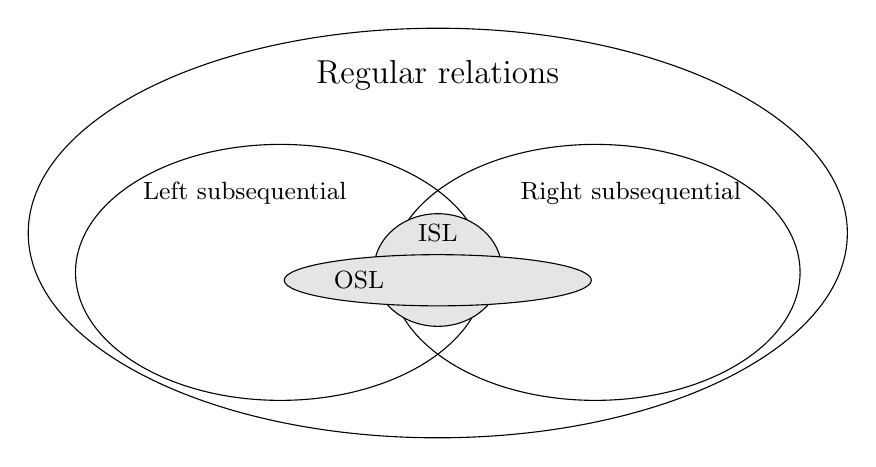
\begin{tikzpicture}
\small    
	\draw (0,0) ellipse (16em and 8em);
    \node at (0,2) {\large Regular relations};
    %
    \draw (-2,-0.5) ellipse (8em and 5em);
    \node at (-2.45,0.5) {Left subsequential};
    %
    \draw (2,-0.5) ellipse (8em and 5em);
    \node at (2.45,0.5) {Right subsequential};
    %
    \draw[black,fill=gray!20] (0, -0.47) ellipse (2.5em and 2.2em);
    \node at (0,0) {ISL};
    %
    \draw[black,fill=gray!20] (0, -0.6) ellipse (6em and 1em);
    \node at (-1,-0.6) {OSL};
\end{tikzpicture}
\caption{Relationship among left subsequential, right subsequential, OSL, and ISL functions; adapted and simplified from \citep{Chandlee2014}.}
\label{fig:ssqfunctionsmanyy}
\end{center}
\end{figure}





\cite{ChandleeEtAl2014} define both ISL and OSL mappings using the notion of \textbf{tails}.
Tails show the dependency between the possible continuations of input strings, and portions of the output contributed by those continuations.
Formally, tails are defined as $tails(x) = \{(y, v) : f(x\cdot y) = u\cdot v \textrm{ and } u = lcp(f(x\cdot \Sigma^*))\}$, where $f$ is the function mapping the input strings to the corresponding outputs, $\cdot$ is the concatenation operator, and $lcp$ is the longest common prefix.
For example, the longest common prefix of $abc$ and $abde$ is $ab$, since it is the longest prefix shared by those two strings.
A slightly extended notation introduced below changes that definition to $tails(\vv{\bm{x}}) = \{(y, v) : f(\vv{\bm{x}}\cdot y) = \bm{u}\cdot v \textrm{ and } u = lcp(f(\vv{\bm{x}}\cdot \Sigma^*))\}$.



Assume that $\Sigma$ and $\Gamma$ are (possibly different) alphabets used to represent the strings before and after application of some rule.
Additionally, strings $\vv{\bm{x}}$ and $y$ belong to $\Sigma^*$, and $\bm{u}$ and $v$ belong to $\Gamma^*$, i.e.\ these strings consist only of symbols included in $\Sigma^*$ or $\Gamma^*$, respectively.
A tail of the prefix $\vv{\bm{x}}$ is a list of all pairs $(y, v)$, where $y$ is a possible continuation of the input prefix $\vv{\bm{x}}$, i.e.\ $\vv{\bm{x}}\cdot y$ is the input string.
The corresponding to $\vv{\bm{x}}\cdot y$ output string is $\bm{u}\cdot v$, where $\bm{u}$ is the longest prefix shared by all outputs corresponding to inputs starting with $\vv{\bm{x}}$.


As an example, let us find a list of tails of the input prefix $\vv{\bm{\bow aa}}$ in the mapping $M$.
Note, that only the input strings are annotated with the edges $\bow$ and $\eow$.


\begin{multline*}
M = (\bow aa\eow, aa), (\bow aaa\eow, aba), (\bow aaaa\eow, abba), (\bow aaaaa\eow, abbba), \\
 \qquad\quad \shoveleft{(\bow aaaaaa\eow, abbbba), (\bow aaaaaaa\eow, abbbbba)\dots}
\end{multline*}


All input strings of that mapping start with $\vv{\bm{\bow aa}}$.
The longest common prefix of the corresponding output strings is $\bm{a}$: for example, the second symbol is different in $aa$ and $aba$.
Below, I mark the selected input prefix $\vv{\bm{\bow aa}}$ and the longest common prefix $\bm{a}$.


$$
M_{marked} = (\vv{\bm{\bow aa}}\eow, \bm{a}a), (\vv{\bm{\bow aa}}a\eow, \bm{a}ba), (\vv{\bm{\bow aa}}aa\eow, \bm{a}bba), (\vv{\bm{\bow aa}}aaa\eow, \bm{a}bbba) \dots
$$

The list of tails of $\vv{\bm{\bow aa}}$ can be computed by removing $\vv{\bm{\bow aa}}$ and $\bm{a}$ from the input and output strings of $M_{marked}$, respectively.

$$
tails(\vv{\bm{\bow aa}}) = (\eow, a), (a\eow, ba), (aa\eow, bba), (aaa\eow, bbba)\dots
$$

The obtained list of tails implies that after observing $\vv{\bm{\bow aa}}$, the input continuation $\eow$ introduces $a$ to the translation,  $a\eow$ contributes $ba$, and so on.
Further in this subsection, I show how the notion of tails is used to define ISL and OSL mappings \citep{Chandlee2014,ChandleeEtAl2014,ChandleeEtAl2015}.



\subsubsection{Input strictly local mappings}

The $k$-ISL functions encode simultaneous rule application, i.e.\ when a transformational rule applied to all positions at the same time.
In mapping $M$, for example, $a$ is substituted by $b$ if it is surrounded by $a$ \emph{in the input string}.
It creates pairs such as $(aaaaa, abbba)$: three internal $a$ 
are changed to $b$ since their context in the input string is the same as specified by the rule $a \rightarrow b / a~ \_~ a$.

\cite{ChandleeEtAl2014} define an ISL mapping as follows.
If two input strings $u_1$ and $u_2$ share the same $k-1$-local suffix, their set of tails is identical as well.

\[
	\textrm{\emph{suff}}^{k-1}(u_1) = \textrm{\emph{suff}}^{k-1}(u_2) \Rightarrow~ tails(u_1) = tails(u_2)
\]

If the mapping $M$ is indeed ISL, the set of tails is the same for all strings ending with the same $k-1$ local prefix.
Let us assume that $k=3$, since the rule targets an item in the context of two other elements.
Input strings $\bow aa\eow$ and $\bow aaa\eow$ both have the $2$-local suffix $a\eow$, and that definition states that their sets of tails must be identical as well.
To confirm this, let us compare tails of $\bow aa$ and $\bow aaa$.


\begin{multline*}
tails(\vv{\bm{\bow aa}}) = (\vv{\bm{\bow aa}}\eow, \bm{a}a), (\vv{\bm{\bow aa}}a\eow, \bm{a}ba), (\vv{\bm{\bow aa}}aa\eow, \bm{a}bba) \dots~ =  \\
 \qquad\qquad\qquad\qquad\quad \shoveleft{(\eow, a), (a\eow, ba), (aa\eow, bba) \dots}
\end{multline*}

\begin{multline*}
tails(\vv{\bm{\bow aaa}}) = (\vv{\bm{\bow aaa}}\eow, \bm{ab}a), (\vv{\bm{\bow aaa}}a\eow, \bm{ab}ba), (\vv{\bm{\bow aaa}}aa\eow, \bm{ab}bba) \dots~ =  \\
 \qquad\qquad\qquad\qquad\quad \shoveleft{(\eow, a), (a\eow, ba), (aa\eow, bba) \dots}
\end{multline*}

Their tails are indeed the same, and it confirms that the \emph{simultaneous application} of the rule $a \rightarrow b / a~ \_~ a$ is an \emph{ISL} function.
The corresponding transducer encodes a $3$-local window reading the input string.
Knowledge of the previous $2$ input symbols informs the transducer about the next action regarding the following symbol that it reads.
Figure \ref{fig:fwoeirwj} demonstrates these steps.

\begin{figure}[h!]
\begin{center}
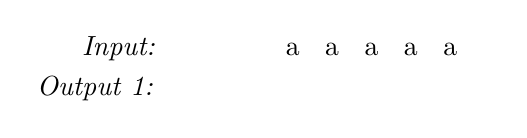
\begin{tikzpicture}
\node at (-1.7,0.25) {\emph{Input:}};
\node (0) at (0,0.25) {$\rtimes$};
\node (1) at (0.5,0.25) {a};
\node (2) at (1,0.25) {a};
\node (3) at (1.5,0.25) {a};
\node (4) at (2,0.25) {a};
\node (5) at (2.5,0.25) {a};
\node (6) at (3,0.25) {$\ltimes$};
%
\node at (-2,-0.25) {\emph{Output 1:}};
\node (0) at (0,-0.25) {$\rtimes$};
\end{tikzpicture}
\vspace{0.5em}

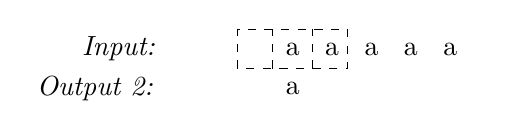
\begin{tikzpicture}
\node at (-1.7,0.25) {\emph{Input:}};
\node (0) at (0,0.25) {$\rtimes$};
\node (1) at (0.5,0.25) {a};
\node (2) at (1,0.25) {a};
\node (3) at (1.5,0.25) {a};
\node (4) at (2,0.25) {a};
\node (5) at (2.5,0.25) {a};
\node (6) at (3,0.25) {$\ltimes$};
%
\node at (-2,-0.25) {\emph{Output 2:}};
\node (0) at (0,-0.25) {$\rtimes$};
\node (01) at (0.5,-0.25) {a};
%
\draw [dashed] (-0.2,0) -- (-0.2,0.5) -- (1.2,0.5) -- (1.2,0) -- (-0.2,0);
\draw [dashed] (0.25, 0) -- (0.25, 0.5);
\draw [dashed] (0.75, 0) -- (0.75, 0.5);
\end{tikzpicture}
\vspace{0.5em}

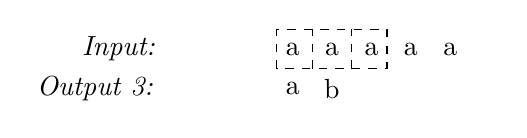
\begin{tikzpicture}
\node at (-1.7,0.25) {\emph{Input:}};
\node (0) at (0,0.25) {$\rtimes$};
\node (1) at (0.5,0.25) {a};
\node (2) at (1,0.25) {a};
\node (3) at (1.5,0.25) {a};
\node (4) at (2,0.25) {a};
\node (5) at (2.5,0.25) {a};
\node (6) at (3,0.25) {$\ltimes$};
%
\node at (-2,-0.25) {\emph{Output 3:}};
\node (0) at (0,-0.25) {$\rtimes$};
\node (01) at (0.5,-0.25) {a};
\node (01) at (1,-0.25) {b};
%
\draw [dashed] (-0.2+0.5,0) -- (-0.2+0.5,0.5) -- (1.2+0.5,0.5) -- (1.2+0.5,0) -- (-0.2+0.5,0);
\draw [dashed] (0.25+0.5, 0) -- (0.25+0.5, 0.5);
\draw [dashed] (0.75+0.5, 0) -- (0.75+0.5, 0.5);
\end{tikzpicture}
\vspace{0.5em}

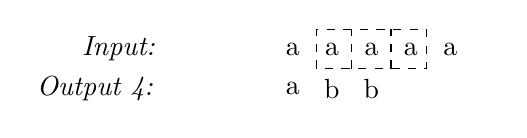
\begin{tikzpicture}
\node at (-1.7,0.25) {\emph{Input:}};
\node (0) at (0,0.25) {$\rtimes$};
\node (1) at (0.5,0.25) {a};
\node (2) at (1,0.25) {a};
\node (3) at (1.5,0.25) {a};
\node (4) at (2,0.25) {a};
\node (5) at (2.5,0.25) {a};
\node (6) at (3,0.25) {$\ltimes$};
%
\node at (-2,-0.25) {\emph{Output 4:}};
\node (0) at (0,-0.25) {$\rtimes$};
\node (01) at (0.5,-0.25) {a};
\node (01) at (1,-0.25) {b};
\node (01) at (1.5,-0.25) {b};
%
\draw [dashed] (-0.2+1,0) -- (-0.2+1,0.5) -- (1.2+1,0.5) -- (1.2+1,0) -- (-0.2+1,0);
\draw [dashed] (0.25+1, 0) -- (0.25+1, 0.5);
\draw [dashed] (0.75+1, 0) -- (0.75+1, 0.5);
\end{tikzpicture}
\vspace{0.5em}

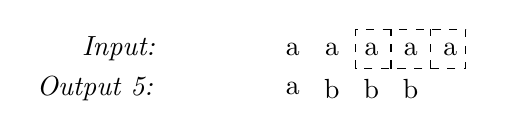
\begin{tikzpicture}
\node at (-1.7,0.25) {\emph{Input:}};
\node (0) at (0,0.25) {$\rtimes$};
\node (1) at (0.5,0.25) {a};
\node (2) at (1,0.25) {a};
\node (3) at (1.5,0.25) {a};
\node (4) at (2,0.25) {a};
\node (5) at (2.5,0.25) {a};
\node (6) at (3,0.25) {$\ltimes$};
%
\node at (-2,-0.25) {\emph{Output 5:}};
\node (0) at (0,-0.25) {$\rtimes$};
\node (01) at (0.5,-0.25) {a};
\node (01) at (1,-0.25) {b};
\node (01) at (1.5,-0.25) {b};
\node (01) at (2,-0.25) {b};
%
\draw [dashed] (-0.2+1.5,0) -- (-0.2+1.5,0.5) -- (1.2+1.5,0.5) -- (1.2+1.5,0) -- (-0.2+1.5,0);
\draw [dashed] (0.25+1.5, 0) -- (0.25+1.5, 0.5);
\draw [dashed] (0.75+1.5, 0) -- (0.75+1.5, 0.5);
\end{tikzpicture}
\vspace{0.5em}

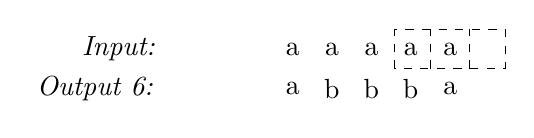
\begin{tikzpicture}
\node at (-1.7,0.25) {\emph{Input:}};
\node (0) at (0,0.25) {$\rtimes$};
\node (1) at (0.5,0.25) {a};
\node (2) at (1,0.25) {a};
\node (3) at (1.5,0.25) {a};
\node (4) at (2,0.25) {a};
\node (5) at (2.5,0.25) {a};
\node (6) at (3,0.25) {$\ltimes$};
%
\node at (-2,-0.25) {\emph{Output 6:}};
\node (0) at (0,-0.25) {$\rtimes$};
\node (01) at (0.5,-0.25) {a};
\node (01) at (1,-0.25) {b};
\node (01) at (1.5,-0.25) {b};
\node (01) at (2,-0.25) {b};
\node (01) at (2.5,-0.25) {a};
%
\draw [dashed] (-0.2+2,0) -- (-0.2+2,0.5) -- (1.2+2,0.5) -- (1.2+2,0) -- (-0.2+2,0);
\draw [dashed] (0.25+2, 0) -- (0.25+2, 0.5);
\draw [dashed] (0.75+2, 0) -- (0.75+2, 0.5);
\end{tikzpicture}
\vspace{0.5em}

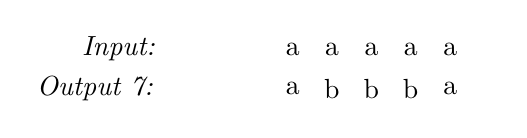
\begin{tikzpicture}
\node at (-1.7,0.25) {\emph{Input:}};
\node (0) at (0,0.25) {$\rtimes$};
\node (1) at (0.5,0.25) {a};
\node (2) at (1,0.25) {a};
\node (3) at (1.5,0.25) {a};
\node (4) at (2,0.25) {a};
\node (5) at (2.5,0.25) {a};
\node (6) at (3,0.25) {$\ltimes$};
%
\node at (-2,-0.25) {\emph{Output 7:}};
\node (0) at (0,-0.25) {$\rtimes$};
\node (01) at (0.5,-0.25) {a};
\node (01) at (1,-0.25) {b};
\node (01) at (1.5,-0.25) {b};
\node (01) at (2,-0.25) {b};
\node (01) at (2.5,-0.25) {a};
\node (6) at (3,-0.25) {$\ltimes$};
\end{tikzpicture}
\caption{ISL application of the rule $a \rightarrow b / a~ \_~ a$ to \emph{aaaaa}.}
\label{fig:fwoeirwj}
\end{center}
\end{figure}

\subsubsection{Output strictly local mappings}

Now, let us consider the iterative application of the same rule $a \rightarrow b / a~ \_~ a$.
In this case, every time the rule is applied, it changes the form that the same rule produced earlier, and therefore $aaaaa$ is changed to $ababa$.
This type of transformation can be visualized as a $3$-local window moving through the input string and rewriting the middle item if the contexts match.
The steps below show the application of the rule; the underlined segments are the contexts, and the boxed items show how the target element was changed.
The list of pairs in $M'$ shows the corresponding mapping.

$$
\underline{\bow}\dbox{a:a}\underline{a}aaa\eow~ \rightarrow
\bow\underline{a}\dbox{a:b}\underline{a}aa\eow~ \rightarrow
\bow a\underline{b}\dbox{a:a}\underline{a}a\eow~ \rightarrow
\bow ab\underline{a}\dbox{a:b}\underline{a}\eow~ \rightarrow
\bow aba\underline{b}\dbox{a:a}\underline{\eow}
$$

\begin{multline*}
M' = (\bow aa\eow, aa), (\bow aaa\eow, aba), (\bow aaaa\eow, abaa), (\bow aaaaa\eow, ababa), \\
 \qquad\quad \shoveleft{(\bow aaaaaa\eow, ababaa), (\bow aaaaaaa\eow, abababa)\dots}
\end{multline*}

\cite{ChandleeEtAl2015} shows that such mappings are $k$-OSL since the previous application of this rule affects the following one.
Their definition of OSL mappings is below, where the function $f$, as previously, maps its argument (input string) to the corresponding output.
For a mapping to be OSL, the following needs to be true: if two output strings share the same $k-1$-local suffix, the tails of the corresponding input strings are the same.


\[
	suff^{k-1}(f(u_1)) = suff^{k-1}(f(u_2)) \Rightarrow~ tails(u_1) = tails(u_2)
\]

That would imply that in the mapping $M'$, tails of $\vv{\bm{\bow aaa}}$ and $\vv{\bm{\bow aaaaa}}$ are the same because the translations of $\bow aaa\eow$ and $\bow aaaaa\eow$ share the same $k-1$-local suffix $ba$ (those translations are $aba$ and $ababa$, respectively).

\begin{multline*}
tails(\vv{\bm{\bow aaa}}) = (\vv{\bm{\bow aaa}}\eow, \bm{aba}), (\vv{\bm{\bow aaa}}a\eow, \bm{aba}a), (\vv{\bm{\bow aaa}}aa\eow, \bm{aba}ba) \dots~ =  \\
 \qquad\qquad\qquad\qquad\quad \shoveleft{(\eow, \varepsilon), (a\eow, a), (aa\eow, ba) \dots}
\end{multline*}

\begin{multline*}
tails(\vv{\bm{\bow aaaaa}}) = \\
\qquad \shoveleft{(\vv{\bm{\bow aaaaa}}\eow, \bm{ababa}), (\vv{\bm{\bow aaaaa}}a\eow, \bm{ababa}a), (\vv{\bm{\bow aaaaa}}aa\eow, \bm{ababa}ba) \dots~ =}  \\
 \qquad\qquad\qquad\qquad\quad \shoveleft{(\eow, \varepsilon), (a\eow, a), (aa\eow, ba) \dots}
\end{multline*}

Indeed, since their tails are the same, this shows that the mapping is OSL.
The corresponding transducer encodes a $3$-local window that keeps track of the last $2$ output symbols.
Based on those symbols and the current symbol it decides how that current symbol is changed.
The iterative rule application is demonstrated in Figure \ref{fig:dgsldkgjsd}.



\begin{figure}[t]
\begin{center}
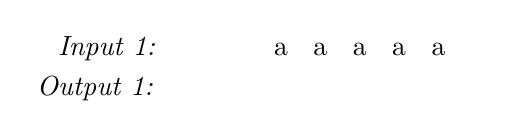
\begin{tikzpicture}
\node at (-1.7,0.25) {\emph{Input 1:}};
\node (0) at (0,0.25) {$\rtimes$};
\node (1) at (0.5,0.25) {a};
\node (2) at (1,0.25) {a};
\node (3) at (1.5,0.25) {a};
\node (4) at (2,0.25) {a};
\node (5) at (2.5,0.25) {a};
\node (6) at (3,0.25) {$\ltimes$};
%
\node at (-1.85,-0.25) {\emph{Output 1:}};
\node (0) at (0,-0.25) {$\rtimes$};
\end{tikzpicture}
\vspace{0.5em}

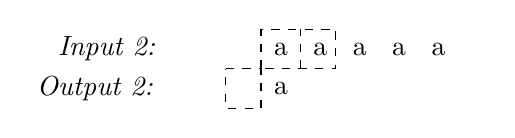
\begin{tikzpicture}
\node at (-1.7,0.25) {\emph{Input 2:}};
\node (0) at (0,0.25) {$\rtimes$};
\node (1) at (0.5,0.25) {a};
\node (2) at (1,0.25) {a};
\node (3) at (1.5,0.25) {a};
\node (4) at (2,0.25) {a};
\node (5) at (2.5,0.25) {a};
\node (6) at (3,0.25) {$\ltimes$};
%
\node at (-1.85,-0.25) {\emph{Output 2:}};
\node (0) at (0,-0.25) {$\rtimes$};
\node (01) at (0.5,-0.25) {a};
%
\draw [dashed] (0.25,0) -- (0.25,0.5) -- (1.2,0.5) -- (1.2,0) -- (0.25,0);
\draw [dashed] (-0.2, 0) -- (0.25, 0) -- (0.25, -0.5) -- (-0.2, -0.5) -- (-0.2, 0);
\draw [dashed] (0.75, 0) -- (0.75, 0.5);
\end{tikzpicture}
\vspace{0.5em}

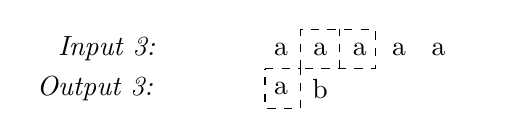
\begin{tikzpicture}
\node at (-1.7,0.25) {\emph{Input 3:}};
\node (0) at (0,0.25) {$\rtimes$};
\node (1) at (0.5,0.25) {a};
\node (2) at (1,0.25) {a};
\node (3) at (1.5,0.25) {a};
\node (4) at (2,0.25) {a};
\node (5) at (2.5,0.25) {a};
\node (6) at (3,0.25) {$\ltimes$};
%
\node at (-1.85,-0.25) {\emph{Output 3:}};
\node (0) at (0,-0.25) {$\rtimes$};
\node (01) at (0.5,-0.25) {a};
\node (01) at (1,-0.25) {b};
%
\draw [dashed] (0.25 + 0.5,0) -- (0.25 + 0.5,0.5) -- (1.2 + 0.5,0.5) -- (1.2 + 0.5,0) -- (0.25 + 0.5,0);
\draw [dashed] (-0.2 + 0.5, 0) -- (0.25 + 0.5, 0) -- (0.25 + 0.5, -0.5) -- (-0.2 + 0.5, -0.5) -- (-0.2 + 0.5, 0);
\draw [dashed] (0.75 + 0.5, 0) -- (0.75 + 0.5, 0.5);
\end{tikzpicture}
\vspace{0.5em}

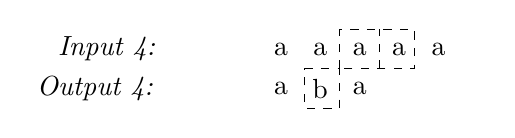
\begin{tikzpicture}
\node at (-1.7,0.25) {\emph{Input 4:}};
\node (0) at (0,0.25) {$\rtimes$};
\node (1) at (0.5,0.25) {a};
\node (2) at (1,0.25) {a};
\node (3) at (1.5,0.25) {a};
\node (4) at (2,0.25) {a};
\node (5) at (2.5,0.25) {a};
\node (6) at (3,0.25) {$\ltimes$};
%
\node at (-1.85,-0.25) {\emph{Output 4:}};
\node (0) at (0,-0.25) {$\rtimes$};
\node (01) at (0.5,-0.25) {a};
\node (01) at (1,-0.25) {b};
\node (01) at (1.5,-0.25) {a};
%
\draw [dashed] (0.25 + 1,0) -- (0.25 + 1,0.5) -- (1.2 + 1,0.5) -- (1.2 + 1,0) -- (0.25 + 1,0);
\draw [dashed] (-0.2 + 1, 0) -- (0.25 + 1, 0) -- (0.25 + 1, -0.5) -- (-0.2 + 1, -0.5) -- (-0.2 + 1, 0);
\draw [dashed] (0.75 + 1, 0) -- (0.75 + 1, 0.5);
\end{tikzpicture}
\vspace{0.5em}

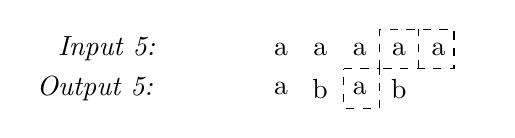
\begin{tikzpicture}
\node at (-1.7,0.25) {\emph{Input 5:}};
\node (0) at (0,0.25) {$\rtimes$};
\node (1) at (0.5,0.25) {a};
\node (2) at (1,0.25) {a};
\node (3) at (1.5,0.25) {a};
\node (4) at (2,0.25) {a};
\node (5) at (2.5,0.25) {a};
\node (6) at (3,0.25) {$\ltimes$};
%
\node at (-1.85,-0.25) {\emph{Output 5:}};
\node (0) at (0,-0.25) {$\rtimes$};
\node (01) at (0.5,-0.25) {a};
\node (01) at (1,-0.25) {b};
\node (01) at (1.5,-0.25) {a};
\node (01) at (2,-0.25) {b};
%
\draw [dashed] (0.25 + 1.5,0) -- (0.25 + 1.5,0.5) -- (1.2 + 1.5,0.5) -- (1.2 + 1.5,0) -- (0.25 + 1.5,0);
\draw [dashed] (-0.2 + 1.5, 0) -- (0.25 + 1.5, 0) -- (0.25 + 1.5, -0.5) -- (-0.2 + 1.5, -0.5) -- (-0.2 + 1.5, 0);
\draw [dashed] (0.75 + 1.5, 0) -- (0.75 + 1.5, 0.5);
\end{tikzpicture}
\vspace{0.5em}

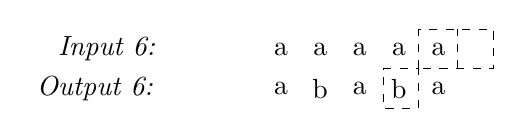
\begin{tikzpicture}
\node at (-1.7,0.25) {\emph{Input 6:}};
\node (0) at (0,0.25) {$\rtimes$};
\node (1) at (0.5,0.25) {a};
\node (2) at (1,0.25) {a};
\node (3) at (1.5,0.25) {a};
\node (4) at (2,0.25) {a};
\node (5) at (2.5,0.25) {a};
\node (6) at (3,0.25) {$\ltimes$};
%
\node at (-1.85,-0.25) {\emph{Output 6:}};
\node (0) at (0,-0.25) {$\rtimes$};
\node (01) at (0.5,-0.25) {a};
\node (01) at (1,-0.25) {b};
\node (01) at (1.5,-0.25) {a};
\node (01) at (2,-0.25) {b};
\node (01) at (2.5,-0.25) {a};
%
\draw [dashed] (0.25 + 2,0) -- (0.25 + 2,0.5) -- (1.2 + 2,0.5) -- (1.2 + 2,0) -- (0.25 + 2,0);
\draw [dashed] (-0.2 + 2, 0) -- (0.25 + 2, 0) -- (0.25 + 2, -0.5) -- (-0.2 + 2, -0.5) -- (-0.2 + 2, 0);
\draw [dashed] (0.75 + 2, 0) -- (0.75 + 2, 0.5);
\end{tikzpicture}
\vspace{0.5em}

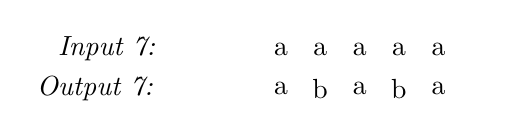
\begin{tikzpicture}
\node at (-1.7,0.25) {\emph{Input 7:}};
\node (0) at (0,0.25) {$\rtimes$};
\node (1) at (0.5,0.25) {a};
\node (2) at (1,0.25) {a};
\node (3) at (1.5,0.25) {a};
\node (4) at (2,0.25) {a};
\node (5) at (2.5,0.25) {a};
\node (6) at (3,0.25) {$\ltimes$};
%
\node at (-1.85,-0.25) {\emph{Output 7:}};
\node (0) at (0,-0.25) {$\rtimes$};
\node (01) at (0.5,-0.25) {a};
\node (01) at (1,-0.25) {b};
\node (01) at (1.5,-0.25) {a};
\node (01) at (2,-0.25) {b};
\node (01) at (2.5,-0.25) {a};
\node (6) at (3,-0.25) {$\ltimes$};
\end{tikzpicture}

\caption{OSL application of the rule $a \rightarrow b / a~ \_~ a$ to \emph{aaaaa}.}
\label{fig:dgsldkgjsd}
\end{center}
\end{figure}




To sum up, $k$-ISL and $k$-OSL mappings encode dependencies affecting $k$-local windows.
ISL functions apply a rule simultaneously to all the positions of the input string, whereas the OSL functions apply a rule step-by-step.
While in the former case, the changes are independent from each other, the latter uses information about the previous change to inform the following one.
\cite{Chandlee2014} argues that linguistic strictly local processes are ISL or OSL, and demonstrates it using a variety of linguistic examples such as Greek fricative deletion, English flapping, and others \citep{JosephPhilippakiWarburton1987}.




\subsection{Models of transformations: summary}


FSTs encode regular mappings that are well-known to be a good fit for natural language phonology and morphology \citep{Johnson1972,KaplanKay94,BeesleyKartunnen03}.
However, a particular class of functions, namely, \emph{subsequential}, includes the major part of natural language patterns.
Transducers implementing subsequential mappings read the symbols of the underlying representations one by one and output the corresponding surface forms.
This allows one to model a wide variety of local and long-distance dependencies such as word-final devoicing and vowel harmony.
For the discussion of predictions and outcomes of subregular and subsequential modeling, see Section~ 2.2.2.

It should be noted that some attested phonological processes are not subsequential.
Among them, there are circumambient pattern of unbounded tonal plateauing and reduplication requiring the power of two-way FSTs \citep{Jardine2016,DolatianHeinz2018}.
Those patterns, however, are beyond the scope of this dissertation.


In Chapter 4, I discuss results of tool-assisted learning experiments targeting various phonological processes such as tone plateauing, local processes, and different types of harmony systems with and without blockers.





\section{Learning grammars from data}
\label{learningframework}


Previous sections showed that subregular grammars can model natural language dependencies.
However, all the previously presented grammars were constructed manually.
In this section, I discuss the possibility of building those models \emph{automatically}.
It not only allows the researchers to avoid the burden of manual grammar construction, but also gives us insights into the mechanisms helping to discover those patters.


\emph{Grammatical inference} is a sub-field of machine learning 
that is concerned with the extraction of grammars from data.
As Colin de la Higuera formulates in his book ``Grammatical Inference'' (\citeyear{DeLaHiguera2010}), this field lies at the intersection of linguistics, inductive analysis, and pattern recognition.
\emph{Linguistics}, and computational linguistics, in particular, brings the core idea of the existence of a \emph{formal grammar}, or a set of rules defining a \emph{language}.
\emph{Language learning} can then be viewed as a process of discovering a language's grammar by the learner.
The field of \emph{inductive inference} aims at a problem of inferring the underlying grammar that consistently predicts what is grammatical and what is not after observing a set of elements of the language, where those elements can be strings, trees, or other structured objects.
Finally, \emph{pattern recognition} describes the best model and its properties that would explain the data; it \emph{analyzes} the pattern.

If the task is to model a language, then the goal is to find a grammar that describes that language.
If the grammar is not known \emph{a priori}, it might be possible to \emph{learn} its rules by observing and exploring the language.
\textbf{Grammatical inference algorithms} require a finite sample of data representing the target language as input, and return a grammar hypothesis as output.
Often, such algorithms need only \textbf{positive data}, or, in other words, a collection of well-formed structures of the target language.
However, some algorithms require \textbf{negative data} as well --- in this case, a list of ill-formed words needs to be available.
That grammar solves a \textbf{membership problem} for that language, or, in other words, it correctly predicts for any given string if that string belongs to the target language, see Figure \ref{fig:LGrel}.
If instead a mapping needs to be learned, grammatical inference algorithms require a sufficient sample of the input-output pairs as input and construct a transducer that generalizes that mapping.

\begin{figure}[t]
  \centering
  \begin{tikzpicture}
  \small
    \draw (0.3,0.2) circle (0.92cm);
    \draw (0,0) circle (2cm);
    \draw (5,0) -- (5.5,0.7) -- (7.5,0.7) -- (8,0) -- (7.5,-0.7) -- (5.5,-0.7) -- (5,0);
    \draw[-{Latex[length=3mm]}] (0.97,0.8) arc (150:28.5:3cm);
    \draw[-{Latex[length=3mm]}] (6,-0.7) arc (-20:-146:2.5cm);
    
    \path (0.35,0.2) node[text width=1.5cm,align=center] {\baselineskip=10pt finite sample \\ of $\mathcal{L}$};
    \path (0, -1.3) node[text width=2cm,align=center] {\baselineskip=10pt language $\mathcal{L}$};
    \path (6.5, 0) node[text width=2cm,align=center] {\baselineskip=10pt grammar $\mathcal{G}$};
    \path (3.5, 2.6) node[text width=4cm,align=center] {\baselineskip=10pt grammatical inference};
     \path (3.5,-2.65) node[text width=4cm,align=center] {\baselineskip=10pt membership problem};
  \end{tikzpicture}
  \caption{Relationship between a language $\mathcal{L}$ and a grammar $\mathcal{G}$.}
  \label{fig:LGrel}
\end{figure}


The learning algorithms for SL, SP, TSL and MTSL languages, and also the algorithm inferring subsequential mappings, will be discussed in details in Chapters 3 and 4.
These algorithms share several common properties: they all require only positive data to find the grammar, they are fully interpretable, and work in polynomial time and data.
In what follows, I explain these properties.
Indeed, \emph{learning only from the positive data} is the desired characteristic, since human learners do not have access to what is not possible in their languages: a finite sample of well-formed examples is sufficient for extracting the pattern. \citep{Chomsky1986}.
Only some of the subregular languages have this property: the full class of regular languages cannot be learned from positive data.
\emph{Interpretability} of an algorithm means that both the learning process and the outcome are transparent: it is possible to trace how the learner came to a certain conclusion, and explain the obtained results.
These learners extract grammars in \emph{polynomial time}, so they can be computed in practice.
(The running time of polynomial algorithms is $n^c$, where $n$ is the size of the training sample, and $c$ is some constant \citep{Sipser2013}.)
Finally, \emph{learning in the limit} guarantees that after a finite number of errors, the learner will start making only correct predictions \citep{Gold1967}. 

As a part of my dissertation, I implemented the \emph{SigmaPie} package \href{https://pypi.org/project/SigmaPie/}{\faCube} for working with subregular languages and mappings.
It provides learners for SL, TSL, MTSL, SP languages and subsequential mappings \citep{sigmapie}.
In Chapter 3, I explore how well those subregular learners extract \emph{well-formedness conditions} from artificial automatically generated datasets exhibiting human language-like patterns such as one or more harmonies with or without blockers, word-final devoicing, tone plateauing, and others.
The training sample for those experiments is a collection of words well-formed according to one of those generalizations.
Later in Chapter 4, I explore modeling of \emph{processes} similar to the ones listed above.
In this case, the training sample contains pairs of underlying representations and the corresponding surface forms.
In such a way, I model processes and well-formedness conditions using tools implemented as a part of \emph{SigmaPie}.


\section{Aspects of practical applications}
\label{aspects}


There were several successful applications of grammatical inference algorithms in the previous decades.
For example, Alexander Clark won the Tenjinno competition in 2006 by using a modified version of OSTIA, a subsequential learner discussed further in Chapter 4 \citep{OncinaEtAl1993,Clark2006}.
Also, \cite{Chandlee-FuEtAl-2012-IGIRP} explore the integration of FSA-based grammatical inference techniques into robotic planning.


However, the subregular learners are \emph{structural} and not probabilistic, and therefore frequently, the absence of some particular configuration in the training sample results in the algorithm failing to learn simple patterns.
For instance, \cite{GildeaJurafsky1996} show that a corpus of English pronunciations is not enough for OSTIA to generalize a rule of English flapping.


Indeed, the results of my Chapters 3 and 4 confirm that local restrictions and gaps in the natural language data obscure the extraction of some dependencies.
This is why I mostly focused on learning \emph{sub-phenomena} instead of the complex interactions of local and long-distance dependencies found in natural language data.
Alternatively, capturing different aspects of the data can be done by combining forces of different learners \citep{Heinz10ldp,HeinzIdsardi13}.
For example, a language can exhibit tone plateauing (SP) together with a long-distance harmony with blocking (TSL).
To learn this patter, the SP and TSL learning algorithms can be run in parallel, and the intersection of the obtained languages yields the target language.
However, future research is needed to understand if transformations can be combined in a way that would preserve properties such as subsequentiality.


There are other directions of research that could improve the performance of subregular learners.
For example, implementing linguistic notions such as features can help to see the behavior of elements as groups instead of individual segments.
The initial results on integrating features and natural classes are available in \citep{Strother-Garcia-HeinzEtAl-2016-UMTGICSP,chandlee-etal-2019-learning}.
Some prior knowledge about the shape of the data can be encoded into the learners using methods that help to systematically exclude certain possible configurations from consideration, as it was shown by \cite{WellmanHenrion1993}.
Also, adding probabilities to the learning algorithms allows abandoning the ``black and white'' structural approach incapable of modeling such probabilistic phenomena as harmony fading or the occurrence of disharmonic words.
\cite{HeinzRogers2010SPdist,Shibata-Heinz-2019-MLEFRDSL} explore the probabilistic subregular models, and \cite{Heinz-Koirala-2010-MLEFD,VuZehfrooshEtal2018-SRLUSM} add together features and probabilities.

\bigskip\bigskip

This chapter is setting the scene for the automatic modeling of well-formedness conditions and transformational rules using subregular methods.
I introduced the main subclasses of subregular languages and mappings and showed how different typologically diverse linguistic patterns can be captured using subregular means.
It is also worth noticing that subregular classes that seem to be the best fit for linguistic dependencies are also efficiently learnable from positive data.
Moreover, the outcomes of those learning algorithms, as well as the steps of the learning process, are fully interpretable and transparent.
While it requires additional research to understand if subregular languages and mappings provide a tight upper bound on the computational complexity of natural language dependencies, the subregular approach provides valuable perspectives on modeling linguistic phenomena, as discussed in Sections~ 2.1.2 and 2.2.2.
In Chapters 3 and 4, I explore the automatic modeling of linguistic phenomena using subregular learners.